\documentclass[twoside]{book}

% Packages required by doxygen
\usepackage{calc}
\usepackage{doxygen}
\usepackage{graphicx}
\usepackage[utf8]{inputenc}
\usepackage{makeidx}
\usepackage{multicol}
\usepackage{multirow}
\usepackage{fixltx2e}
\PassOptionsToPackage{warn}{textcomp}
\usepackage{textcomp}
\usepackage[nointegrals]{wasysym}
\usepackage[table]{xcolor}

% Font selection
\usepackage[T1]{fontenc}
\usepackage{mathptmx}
\usepackage[scaled=.90]{helvet}
\usepackage{courier}
\usepackage{amssymb}
\usepackage{sectsty}
\renewcommand{\familydefault}{\sfdefault}
\allsectionsfont{%
  \fontseries{bc}\selectfont%
  \color{darkgray}%
}
\renewcommand{\DoxyLabelFont}{%
  \fontseries{bc}\selectfont%
  \color{darkgray}%
}
\newcommand{\+}{\discretionary{\mbox{\scriptsize$\hookleftarrow$}}{}{}}

% Page & text layout
\usepackage{geometry}
\geometry{%
  a4paper,%
  top=2.5cm,%
  bottom=2.5cm,%
  left=2.5cm,%
  right=2.5cm%
}
\tolerance=750
\hfuzz=15pt
\hbadness=750
\setlength{\emergencystretch}{15pt}
\setlength{\parindent}{0cm}
\setlength{\parskip}{0.2cm}
\makeatletter
\renewcommand{\paragraph}{%
  \@startsection{paragraph}{4}{0ex}{-1.0ex}{1.0ex}{%
    \normalfont\normalsize\bfseries\SS@parafont%
  }%
}
\renewcommand{\subparagraph}{%
  \@startsection{subparagraph}{5}{0ex}{-1.0ex}{1.0ex}{%
    \normalfont\normalsize\bfseries\SS@subparafont%
  }%
}
\makeatother

% Headers & footers
\usepackage{fancyhdr}
\pagestyle{fancyplain}
\fancyhead[LE]{\fancyplain{}{\bfseries\thepage}}
\fancyhead[CE]{\fancyplain{}{}}
\fancyhead[RE]{\fancyplain{}{\bfseries\leftmark}}
\fancyhead[LO]{\fancyplain{}{\bfseries\rightmark}}
\fancyhead[CO]{\fancyplain{}{}}
\fancyhead[RO]{\fancyplain{}{\bfseries\thepage}}
\fancyfoot[LE]{\fancyplain{}{}}
\fancyfoot[CE]{\fancyplain{}{}}
\fancyfoot[RE]{\fancyplain{}{\bfseries\scriptsize Generated on Sun Feb 8 2015 18\+:26\+:45 for i\+Robot Roomba 500 Series S\+D\+K by Doxygen }}
\fancyfoot[LO]{\fancyplain{}{\bfseries\scriptsize Generated on Sun Feb 8 2015 18\+:26\+:45 for i\+Robot Roomba 500 Series S\+D\+K by Doxygen }}
\fancyfoot[CO]{\fancyplain{}{}}
\fancyfoot[RO]{\fancyplain{}{}}
\renewcommand{\footrulewidth}{0.4pt}
\renewcommand{\chaptermark}[1]{%
  \markboth{#1}{}%
}
\renewcommand{\sectionmark}[1]{%
  \markright{\thesection\ #1}%
}

% Indices & bibliography
\usepackage{natbib}
\usepackage[titles]{tocloft}
\setcounter{tocdepth}{3}
\setcounter{secnumdepth}{5}
\makeindex

% Hyperlinks (required, but should be loaded last)
\usepackage{ifpdf}
\ifpdf
  \usepackage[pdftex,pagebackref=true]{hyperref}
\else
  \usepackage[ps2pdf,pagebackref=true]{hyperref}
\fi
\hypersetup{%
  colorlinks=true,%
  linkcolor=blue,%
  citecolor=blue,%
  unicode%
}

% Custom commands
\newcommand{\clearemptydoublepage}{%
  \newpage{\pagestyle{empty}\cleardoublepage}%
}


%===== C O N T E N T S =====

\begin{document}

% Titlepage & ToC
\hypersetup{pageanchor=false,
             bookmarks=true,
             bookmarksnumbered=true,
             pdfencoding=unicode
            }
\pagenumbering{roman}
\begin{titlepage}
\vspace*{7cm}
\begin{center}%
{\Large i\+Robot Roomba 500 Series S\+D\+K \\[1ex]\large 1.\+0.\+0-\/alpha }\\
\vspace*{1cm}
{\large Generated by Doxygen 1.8.7}\\
\vspace*{0.5cm}
{\small Sun Feb 8 2015 18:26:45}\\
\end{center}
\end{titlepage}
\clearemptydoublepage
\tableofcontents
\clearemptydoublepage
\pagenumbering{arabic}
\hypersetup{pageanchor=true}

%--- Begin generated contents ---
\chapter{A C++ wrapper for the i\+Robot Roomba Open Interface.}
\label{md___users_zachary_fields__development_bitbucket_irobot-roomba-sdk__r_e_a_d_m_e}
\hypertarget{md___users_zachary_fields__development_bitbucket_irobot-roomba-sdk__r_e_a_d_m_e}{}
\subsection*{S\+A\+M\+P\+L\+E\+S\+:}

$<$ coming soon $>$

\subsection*{T\+O\+D\+O\+:}

$<$ coming soon $>$

\subsection*{A\+T\+T\+R\+I\+B\+U\+T\+I\+O\+N\+:}


\begin{DoxyItemize}
\item The makefiles used for compiling the Google Unit Test where taken from Google.
\end{DoxyItemize}

\subsection*{L\+I\+C\+E\+N\+S\+E\+:}


\begin{DoxyItemize}
\item The M\+I\+T License (M\+I\+T). Refer to the L\+I\+C\+E\+N\+S\+E file for more details. 
\end{DoxyItemize}
\chapter{Namespace Index}
\section{Namespace List}
Here is a list of all documented namespaces with brief descriptions\+:\begin{DoxyCompactList}
\item\contentsline{section}{\hyperlink{namespaceroomba}{roomba} \\*The i\+Robot Roomba autonomous robotic vacuum cleaner }{\pageref{namespaceroomba}}{}
\item\contentsline{section}{\hyperlink{namespaceroomba_1_1serial}{roomba\+::serial} \\*Serial Platform Abstraction Layer }{\pageref{namespaceroomba_1_1serial}}{}
\item\contentsline{section}{\hyperlink{namespaceroomba_1_1state}{roomba\+::state} \\*Constant data used to manage data returned from the i\+Robot® Roomba }{\pageref{namespaceroomba_1_1state}}{}
\end{DoxyCompactList}

\chapter{Hierarchical Index}
\section{Class Hierarchy}
This inheritance list is sorted roughly, but not completely, alphabetically\+:\begin{DoxyCompactList}
\item \contentsline{section}{roomba\+:\+:series500\+:\+:oi\+:\+:O\+I\+Encoder\+:\+:clock\+\_\+time\+\_\+t}{\pageref{structroomba_1_1series500_1_1oi_1_1_o_i_encoder_1_1clock__time__t}}{}
\item \contentsline{section}{roomba\+:\+:series500\+:\+:oi\+:\+:O\+I\+Encoder}{\pageref{classroomba_1_1series500_1_1oi_1_1_o_i_encoder}}{}
\begin{DoxyCompactList}
\item \contentsline{section}{O\+I\+Encoder\+\_\+\+T\+C}{\pageref{class_o_i_encoder___t_c}}{}
\end{DoxyCompactList}
\end{DoxyCompactList}

\chapter{Class Index}
\section{Class List}
Here are the classes, structs, unions and interfaces with brief descriptions\+:\begin{DoxyCompactList}
\item\contentsline{section}{\hyperlink{structroomba_1_1series500_1_1oi_1_1_o_i_encoder_1_1clock__time__t}{roomba\+::series500\+::oi\+::\+O\+I\+Encoder\+::clock\+\_\+time\+\_\+t} \\*Time representation for the scheduling methods }{\pageref{structroomba_1_1series500_1_1oi_1_1_o_i_encoder_1_1clock__time__t}}{}
\item\contentsline{section}{\hyperlink{classroomba_1_1series500_1_1oi_1_1_o_i_encoder}{roomba\+::series500\+::oi\+::\+O\+I\+Encoder} \\*The Roomba Open Interface (O\+I) \hyperlink{classroomba_1_1series500_1_1oi_1_1_o_i_encoder}{O\+I\+Encoder} static class }{\pageref{classroomba_1_1series500_1_1oi_1_1_o_i_encoder}}{}
\item\contentsline{section}{\hyperlink{class_o_i_encoder___t_c}{O\+I\+Encoder\+\_\+\+T\+C} }{\pageref{class_o_i_encoder___t_c}}{}
\end{DoxyCompactList}

\chapter{Namespace Documentation}
\hypertarget{namespaceroomba}{\section{roomba Namespace Reference}
\label{namespaceroomba}\index{roomba@{roomba}}
}


The i\+Robot Roomba autonomous robotic vacuum cleaner.  


\subsection*{Namespaces}
\begin{DoxyCompactItemize}
\item 
 \hyperlink{namespaceroomba_1_1series500}{series500}
\begin{DoxyCompactList}\small\item\em The Roomba 500 Series Model (5xx) \end{DoxyCompactList}\end{DoxyCompactItemize}


\subsection{Detailed Description}
The i\+Robot Roomba autonomous robotic vacuum cleaner. 

Roomba was introduced in 2002. As of Feb 2014, over 10 million units have been sold worldwide. Roomba features a set of basic sensors that help it perform tasks. For instance, the Roomba is able to change direction on encountering obstacles, detect dirty spots on the floor, and detect steep drops to keep it from falling down stairs. It uses two independently operating wheels that allow 360 degree turns. Additionally, it can adapt to perform other more \char`\"{}creative\char`\"{} tasks using an embedded computer in conjunction with the Roomba Open Interface. 
\hypertarget{namespaceroomba_1_1serial}{\section{roomba\+:\+:serial Namespace Reference}
\label{namespaceroomba_1_1serial}\index{roomba\+::serial@{roomba\+::serial}}
}


Serial Platform Abstraction Layer.  


\subsection*{Functions}
\begin{DoxyCompactItemize}
\item 
void \hyperlink{namespaceroomba_1_1serial_a13ea2776b1b20987eac4980cdc194eb5}{begin\+At\+Baud\+Code} (\hyperlink{namespaceroomba_a303ba447b12fc77bc24977a1a7ec6d6c}{roomba\+::\+Baud\+Code} baud\+\_\+code\+\_\+)
\begin{DoxyCompactList}\small\item\em Begin the serial connection. \end{DoxyCompactList}\item 
size\+\_\+t \hyperlink{namespaceroomba_1_1serial_af8bd9971043c83114088d1c43cfd97d4}{delay\+Ms} (const size\+\_\+t desired\+\_\+ms\+\_\+)
\begin{DoxyCompactList}\small\item\em Delay in milliseconds. \end{DoxyCompactList}\item 
size\+\_\+t \hyperlink{namespaceroomba_1_1serial_af7b2e2fc2ec29829a0d72f091d36dcd3}{delay\+Us} (const size\+\_\+t desired\+\_\+us\+\_\+)
\begin{DoxyCompactList}\small\item\em Delay in microseconds. \end{DoxyCompactList}\item 
size\+\_\+t \hyperlink{namespaceroomba_1_1serial_a5f09086cb2b546c2aa5dbd354d981d85}{multi\+Byte\+Serial\+Read} (uint\+\_\+opt8\+\_\+t $\ast$const data\+\_\+buffer\+\_\+, const size\+\_\+t buffer\+\_\+length\+\_\+, const uint\+\_\+opt32\+\_\+t timeout\+\_\+ms\+\_\+=1000)
\begin{DoxyCompactList}\small\item\em A function supplying multi-\/byte read access to the serial bus. \end{DoxyCompactList}\item 
size\+\_\+t \hyperlink{namespaceroomba_1_1serial_a5700ad1549232f61cdcecfdf8f480cf3}{multi\+Byte\+Serial\+Write} (const uint\+\_\+opt8\+\_\+t $\ast$const serial\+\_\+data\+\_\+, const size\+\_\+t data\+\_\+length\+\_\+)
\begin{DoxyCompactList}\small\item\em A function supplying multi-\/byte write access to the serial bus. \end{DoxyCompactList}\end{DoxyCompactItemize}


\subsection{Detailed Description}
Serial Platform Abstraction Layer. 

This class serves as a serial platform abstraction layer, which lists the basic services to be provided by a serial platform. An explicit serial protocol will be instantiated at compilation. (i.\+e. Wiring, Linux, Windows\+\_\+\+N\+T, Windows\+\_\+\+U\+A\+P, etc...). 

\subsection{Function Documentation}
\hypertarget{namespaceroomba_1_1serial_a13ea2776b1b20987eac4980cdc194eb5}{\index{roomba\+::serial@{roomba\+::serial}!begin\+At\+Baud\+Code@{begin\+At\+Baud\+Code}}
\index{begin\+At\+Baud\+Code@{begin\+At\+Baud\+Code}!roomba\+::serial@{roomba\+::serial}}
\subsubsection[{begin\+At\+Baud\+Code}]{\setlength{\rightskip}{0pt plus 5cm}void roomba\+::serial\+::begin\+At\+Baud\+Code (
\begin{DoxyParamCaption}
\item[{{\bf roomba\+::\+Baud\+Code}}]{baud\+\_\+code\+\_\+}
\end{DoxyParamCaption}
)\hspace{0.3cm}{\ttfamily [inline]}}}\label{namespaceroomba_1_1serial_a13ea2776b1b20987eac4980cdc194eb5}


Begin the serial connection. 

A serial connection will be started at the rate represented by the baud code. 
\begin{DoxyParams}[1]{Parameters}
\mbox{\tt in}  & {\em baud\+\_\+code\+\_\+} & The code indicating a specific rate \\
\hline
\end{DoxyParams}
\hypertarget{namespaceroomba_1_1serial_af8bd9971043c83114088d1c43cfd97d4}{\index{roomba\+::serial@{roomba\+::serial}!delay\+Ms@{delay\+Ms}}
\index{delay\+Ms@{delay\+Ms}!roomba\+::serial@{roomba\+::serial}}
\subsubsection[{delay\+Ms}]{\setlength{\rightskip}{0pt plus 5cm}size\+\_\+t roomba\+::serial\+::delay\+Ms (
\begin{DoxyParamCaption}
\item[{const size\+\_\+t}]{desired\+\_\+ms\+\_\+}
\end{DoxyParamCaption}
)\hspace{0.3cm}{\ttfamily [inline]}}}\label{namespaceroomba_1_1serial_af8bd9971043c83114088d1c43cfd97d4}


Delay in milliseconds. 


\begin{DoxyParams}[1]{Parameters}
\mbox{\tt in}  & {\em desired\+\_\+ms\+\_\+} & The number of milliseconds you wish to wait \\
\hline
\end{DoxyParams}
\begin{DoxyReturn}{Returns}
The actual duration of the delay in milliseconds 
\end{DoxyReturn}
\hypertarget{namespaceroomba_1_1serial_af7b2e2fc2ec29829a0d72f091d36dcd3}{\index{roomba\+::serial@{roomba\+::serial}!delay\+Us@{delay\+Us}}
\index{delay\+Us@{delay\+Us}!roomba\+::serial@{roomba\+::serial}}
\subsubsection[{delay\+Us}]{\setlength{\rightskip}{0pt plus 5cm}size\+\_\+t roomba\+::serial\+::delay\+Us (
\begin{DoxyParamCaption}
\item[{const size\+\_\+t}]{desired\+\_\+us\+\_\+}
\end{DoxyParamCaption}
)\hspace{0.3cm}{\ttfamily [inline]}}}\label{namespaceroomba_1_1serial_af7b2e2fc2ec29829a0d72f091d36dcd3}


Delay in microseconds. 


\begin{DoxyParams}[1]{Parameters}
\mbox{\tt in}  & {\em desired\+\_\+us\+\_\+} & The number of microseconds you wish to wait \\
\hline
\end{DoxyParams}
\begin{DoxyReturn}{Returns}
The actual duration of the delay in microseconds 
\end{DoxyReturn}
\hypertarget{namespaceroomba_1_1serial_a5f09086cb2b546c2aa5dbd354d981d85}{\index{roomba\+::serial@{roomba\+::serial}!multi\+Byte\+Serial\+Read@{multi\+Byte\+Serial\+Read}}
\index{multi\+Byte\+Serial\+Read@{multi\+Byte\+Serial\+Read}!roomba\+::serial@{roomba\+::serial}}
\subsubsection[{multi\+Byte\+Serial\+Read}]{\setlength{\rightskip}{0pt plus 5cm}size\+\_\+t roomba\+::serial\+::multi\+Byte\+Serial\+Read (
\begin{DoxyParamCaption}
\item[{uint\+\_\+opt8\+\_\+t $\ast$const}]{data\+\_\+buffer\+\_\+, }
\item[{const size\+\_\+t}]{buffer\+\_\+length\+\_\+, }
\item[{const uint\+\_\+opt32\+\_\+t}]{timeout\+\_\+ms\+\_\+ = {\ttfamily 1000}}
\end{DoxyParamCaption}
)\hspace{0.3cm}{\ttfamily [inline]}}}\label{namespaceroomba_1_1serial_a5f09086cb2b546c2aa5dbd354d981d85}


A function supplying multi-\/byte read access to the serial bus. 


\begin{DoxyParams}[1]{Parameters}
\mbox{\tt out}  & {\em data\+\_\+buffer\+\_\+} & A buffer used for transfering the contents of the serial bus \\
\hline
\mbox{\tt in}  & {\em buffer\+\_\+length\+\_\+} & The length of the buffer \\
\hline
\mbox{\tt in}  & {\em timeout\+\_\+ms\+\_\+} & The number of milliseconds to wait before returning with a timeout error. \mbox{[}default value\+: 1000\mbox{]} \\
\hline
\end{DoxyParams}
\begin{DoxyReturn}{Returns}
The actual number of bytes placed in the buffer provided 
\end{DoxyReturn}
\hypertarget{namespaceroomba_1_1serial_a5700ad1549232f61cdcecfdf8f480cf3}{\index{roomba\+::serial@{roomba\+::serial}!multi\+Byte\+Serial\+Write@{multi\+Byte\+Serial\+Write}}
\index{multi\+Byte\+Serial\+Write@{multi\+Byte\+Serial\+Write}!roomba\+::serial@{roomba\+::serial}}
\subsubsection[{multi\+Byte\+Serial\+Write}]{\setlength{\rightskip}{0pt plus 5cm}size\+\_\+t roomba\+::serial\+::multi\+Byte\+Serial\+Write (
\begin{DoxyParamCaption}
\item[{const uint\+\_\+opt8\+\_\+t $\ast$const}]{serial\+\_\+data\+\_\+, }
\item[{const size\+\_\+t}]{data\+\_\+length\+\_\+}
\end{DoxyParamCaption}
)\hspace{0.3cm}{\ttfamily [inline]}}}\label{namespaceroomba_1_1serial_a5700ad1549232f61cdcecfdf8f480cf3}


A function supplying multi-\/byte write access to the serial bus. 


\begin{DoxyParams}[1]{Parameters}
\mbox{\tt in}  & {\em serial\+\_\+data\+\_\+} & A serialized data string to be sent on the serial bus \\
\hline
\mbox{\tt in}  & {\em data\+\_\+length\+\_\+} & The length of the data at the pointer passed in the first parameter \\
\hline
\end{DoxyParams}
\begin{DoxyReturn}{Returns}
The actual number of bytes written to the serial bus 
\end{DoxyReturn}

\hypertarget{namespaceroomba_1_1state}{\section{roomba\+:\+:state Namespace Reference}
\label{namespaceroomba_1_1state}\index{roomba\+::state@{roomba\+::state}}
}


Constant data used to manage data returned from the i\+Robot® Roomba.  


\subsection*{Classes}
\begin{DoxyCompactItemize}
\item 
struct \hyperlink{structroomba_1_1state_1_1sensor__data__t}{sensor\+\_\+data\+\_\+t}
\begin{DoxyCompactList}\small\item\em Data structure to overlay sensor blob. \end{DoxyCompactList}\end{DoxyCompactItemize}
\subsection*{Functions}
\begin{DoxyCompactItemize}
\item 
\hyperlink{namespaceroomba_aff53babe0af88b1ea8b066fd18b8f23f}{Return\+Code} \hyperlink{namespaceroomba_1_1state_a85d19eb1f7d2871cf53d0413159b7a2b}{get\+Parse\+Error} (void)
\begin{DoxyCompactList}\small\item\em Accessor method to check for parsing errors. \end{DoxyCompactList}\item 
\hyperlink{namespaceroomba_aff53babe0af88b1ea8b066fd18b8f23f}{Return\+Code} \hyperlink{namespaceroomba_1_1state_a295e713733b669bf36f35aa1304d6af2}{parse\+Query\+Data} (void)
\begin{DoxyCompactList}\small\item\em Function to receive serial data generated by a query command. \end{DoxyCompactList}\item 
\hyperlink{namespaceroomba_aff53babe0af88b1ea8b066fd18b8f23f}{Return\+Code} \hyperlink{namespaceroomba_1_1state_ae7ffae2671309085bfc9e7eacd9cecbe}{parse\+Stream\+Data} (void)
\begin{DoxyCompactList}\small\item\em Function to receive serial data generated by the stream command. \end{DoxyCompactList}\item 
\hyperlink{namespaceroomba_aff53babe0af88b1ea8b066fd18b8f23f}{Return\+Code} \hyperlink{namespaceroomba_1_1state_aea76767beb90c172924534fde3de51f8}{set\+Baud\+Code} (const \hyperlink{namespaceroomba_a303ba447b12fc77bc24977a1a7ec6d6c}{Baud\+Code} baud\+\_\+code\+\_\+)
\begin{DoxyCompactList}\small\item\em Stores the baud code. \end{DoxyCompactList}\item 
\hyperlink{namespaceroomba_aff53babe0af88b1ea8b066fd18b8f23f}{Return\+Code} \hyperlink{namespaceroomba_1_1state_a9c0d2581bdb082ca4603ac8c8cb290a4}{set\+O\+I\+Mode} (const \hyperlink{namespaceroomba_ab6a52ccd26d50ce82376d04a27c6e76a}{O\+I\+Mode} oi\+\_\+mode\+\_\+)
\begin{DoxyCompactList}\small\item\em Stores the operating mode of the Open Interface. \end{DoxyCompactList}\item 
\hyperlink{namespaceroomba_aff53babe0af88b1ea8b066fd18b8f23f}{Return\+Code} \hyperlink{namespaceroomba_1_1state_a67d016785f60c3014347c21ee3b5afe7}{set\+Parse\+Key} (sensor\+::\+Packet\+Id const $\ast$const parse\+\_\+key\+\_\+)
\begin{DoxyCompactList}\small\item\em Function to store parse key. \end{DoxyCompactList}\item 
\hypertarget{namespaceroomba_1_1state_a55a9c0e96dd22e4268531336e5ed2f77}{struct \hyperlink{structroomba_1_1state_1_1sensor__data__t}{roomba\+::state\+::sensor\+\_\+data\+\_\+t} {\bfseries \+\_\+\+\_\+attribute\+\_\+\+\_\+} ((\+\_\+\+\_\+packed\+\_\+\+\_\+))}\label{namespaceroomba_1_1state_a55a9c0e96dd22e4268531336e5ed2f77}

\end{DoxyCompactItemize}


\subsection{Detailed Description}
Constant data used to manage data returned from the i\+Robot® Roomba. 

The state of the i\+Robot Roomba.

Internal helper functions.

This constant data facilitates inserting and retreiving sensor data from the blob. Some \char`\"{}data\char`\"{} is represented \char`\"{}functionally\char`\"{} to reduce wasted space for sparse data sets. The data functions do not contain error checking, and should only be used internally.

Functions used for common calculations. These functions do not supply return codes and are considered to be unsafe.

This namespace provides access to a state machine prescribed by the i\+Robot Roomba Open Interface specification. The namespace stores tracking information when calls are made to set device properties (i.\+e. baud code), it also houses the data returned when the state of the sensors are queried. see \hyperlink{classroomba_1_1_open_interface_a4f90f2d77ee1a99616934bcc63044c97}{Open\+Interface\+::baud} see \hyperlink{classroomba_1_1_open_interface_a414ce50d279ed418660c29196e27f2f2}{Open\+Interface\+::control} see \hyperlink{classroomba_1_1_open_interface_a649c060ea8628d7189d5d588bf224eb4}{Open\+Interface\+::full} see \hyperlink{classroomba_1_1_open_interface_af4e1dfd388fde037cb4a43d1d0e4ab82}{Open\+Interface\+::power} see \hyperlink{classroomba_1_1_open_interface_a4a7308a7119c6a462389d9ffa3785f87}{Open\+Interface\+::query\+List} see \hyperlink{classroomba_1_1_open_interface_a3fe71d50263839dd40838af6adf5f56f}{Open\+Interface\+::safe} see \hyperlink{classroomba_1_1_open_interface_aa676703a4c79547397eaa89ddb9e207c}{Open\+Interface\+::sensors} see \hyperlink{classroomba_1_1_open_interface_a9a55a3f5a4ff10ae6452ffcec6dd80a7}{Open\+Interface\+::start} see \hyperlink{classroomba_1_1_open_interface_af7a1adea482ac71fa9057842a955af6e}{Open\+Interface\+::stream} 

\subsection{Function Documentation}
\hypertarget{namespaceroomba_1_1state_a85d19eb1f7d2871cf53d0413159b7a2b}{\index{roomba\+::state@{roomba\+::state}!get\+Parse\+Error@{get\+Parse\+Error}}
\index{get\+Parse\+Error@{get\+Parse\+Error}!roomba\+::state@{roomba\+::state}}
\subsubsection[{get\+Parse\+Error}]{\setlength{\rightskip}{0pt plus 5cm}{\bf Return\+Code} roomba\+::state\+::get\+Parse\+Error (
\begin{DoxyParamCaption}
\item[{void}]{}
\end{DoxyParamCaption}
)}}\label{namespaceroomba_1_1state_a85d19eb1f7d2871cf53d0413159b7a2b}


Accessor method to check for parsing errors. 

The parsing methods typically execute in a separate thread and is therefore unable to provide return codes directly. This method provides access to the shared memory where the return code is stored. \begin{DoxyReturn}{Returns}
S\+U\+C\+C\+E\+S\+S 

S\+E\+R\+I\+A\+L\+\_\+\+T\+R\+A\+N\+S\+F\+E\+R\+\_\+\+F\+A\+I\+L\+U\+R\+E 
\end{DoxyReturn}
\begin{DoxySeeAlso}{See also}
\hyperlink{namespaceroomba_1_1state_a295e713733b669bf36f35aa1304d6af2}{state\+::parse\+Query\+Data} 

\hyperlink{namespaceroomba_1_1state_ae7ffae2671309085bfc9e7eacd9cecbe}{state\+::parse\+Stream\+Data} 
\end{DoxySeeAlso}
\hypertarget{namespaceroomba_1_1state_a295e713733b669bf36f35aa1304d6af2}{\index{roomba\+::state@{roomba\+::state}!parse\+Query\+Data@{parse\+Query\+Data}}
\index{parse\+Query\+Data@{parse\+Query\+Data}!roomba\+::state@{roomba\+::state}}
\subsubsection[{parse\+Query\+Data}]{\setlength{\rightskip}{0pt plus 5cm}{\bf Return\+Code} roomba\+::state\+::parse\+Query\+Data (
\begin{DoxyParamCaption}
\item[{void}]{}
\end{DoxyParamCaption}
)}}\label{namespaceroomba_1_1state_a295e713733b669bf36f35aa1304d6af2}


Function to receive serial data generated by a query command. 

Parses data received from Roomba and stores it in memory accessible by the O\+I\+Command object. \begin{DoxyReturn}{Returns}
S\+U\+C\+C\+E\+S\+S 

S\+E\+R\+I\+A\+L\+\_\+\+T\+R\+A\+N\+S\+F\+E\+R\+\_\+\+F\+A\+I\+L\+U\+R\+E 
\end{DoxyReturn}
\begin{DoxySeeAlso}{See also}
\hyperlink{classroomba_1_1_open_interface_aa676703a4c79547397eaa89ddb9e207c}{Open\+Interface\+::sensors} 

\hyperlink{classroomba_1_1_open_interface_a4a7308a7119c6a462389d9ffa3785f87}{Open\+Interface\+::query\+List} 
\end{DoxySeeAlso}
\hypertarget{namespaceroomba_1_1state_ae7ffae2671309085bfc9e7eacd9cecbe}{\index{roomba\+::state@{roomba\+::state}!parse\+Stream\+Data@{parse\+Stream\+Data}}
\index{parse\+Stream\+Data@{parse\+Stream\+Data}!roomba\+::state@{roomba\+::state}}
\subsubsection[{parse\+Stream\+Data}]{\setlength{\rightskip}{0pt plus 5cm}{\bf Return\+Code} roomba\+::state\+::parse\+Stream\+Data (
\begin{DoxyParamCaption}
\item[{void}]{}
\end{DoxyParamCaption}
)}}\label{namespaceroomba_1_1state_ae7ffae2671309085bfc9e7eacd9cecbe}


Function to receive serial data generated by the stream command. 

Parses data received from Roomba and stores it in memory accessible by the O\+I\+Command object. \begin{DoxyReturn}{Returns}
S\+U\+C\+C\+E\+S\+S 
\end{DoxyReturn}
\begin{DoxySeeAlso}{See also}
\hyperlink{classroomba_1_1_open_interface_af7a1adea482ac71fa9057842a955af6e}{Open\+Interface\+::stream} 
\end{DoxySeeAlso}
\hypertarget{namespaceroomba_1_1state_aea76767beb90c172924534fde3de51f8}{\index{roomba\+::state@{roomba\+::state}!set\+Baud\+Code@{set\+Baud\+Code}}
\index{set\+Baud\+Code@{set\+Baud\+Code}!roomba\+::state@{roomba\+::state}}
\subsubsection[{set\+Baud\+Code}]{\setlength{\rightskip}{0pt plus 5cm}{\bf Return\+Code} roomba\+::state\+::set\+Baud\+Code (
\begin{DoxyParamCaption}
\item[{const Baud\+Code}]{baud\+\_\+code\+\_\+}
\end{DoxyParamCaption}
)}}\label{namespaceroomba_1_1state_aea76767beb90c172924534fde3de51f8}


Stores the baud code. 

The baud code is used when calculating the time required to execute a sensor query transaction. \begin{DoxyReturn}{Returns}
S\+U\+C\+C\+E\+S\+S 

I\+N\+V\+A\+L\+I\+D\+\_\+\+P\+A\+R\+A\+M\+E\+T\+E\+R 
\end{DoxyReturn}
\begin{DoxySeeAlso}{See also}
\hyperlink{classroomba_1_1_open_interface_aa676703a4c79547397eaa89ddb9e207c}{Open\+Interface\+::sensors} 

\hyperlink{classroomba_1_1_open_interface_a4a7308a7119c6a462389d9ffa3785f87}{Open\+Interface\+::query\+List} 
\end{DoxySeeAlso}
\hypertarget{namespaceroomba_1_1state_a9c0d2581bdb082ca4603ac8c8cb290a4}{\index{roomba\+::state@{roomba\+::state}!set\+O\+I\+Mode@{set\+O\+I\+Mode}}
\index{set\+O\+I\+Mode@{set\+O\+I\+Mode}!roomba\+::state@{roomba\+::state}}
\subsubsection[{set\+O\+I\+Mode}]{\setlength{\rightskip}{0pt plus 5cm}{\bf Return\+Code} roomba\+::state\+::set\+O\+I\+Mode (
\begin{DoxyParamCaption}
\item[{const O\+I\+Mode}]{oi\+\_\+mode\+\_\+}
\end{DoxyParamCaption}
)}}\label{namespaceroomba_1_1state_a9c0d2581bdb082ca4603ac8c8cb290a4}


Stores the operating mode of the Open Interface. 

The variable is used to track the current operating mode of the Roomba's internal state machine (i.\+e. Off, Passive, Safe, Full), and is used as a gate to control available functionality. \begin{DoxyReturn}{Returns}
S\+U\+C\+C\+E\+S\+S 

I\+N\+V\+A\+L\+I\+D\+\_\+\+P\+A\+R\+A\+M\+E\+T\+E\+R see \hyperlink{classroomba_1_1_open_interface_a414ce50d279ed418660c29196e27f2f2}{Open\+Interface\+::control} see \hyperlink{classroomba_1_1_open_interface_a649c060ea8628d7189d5d588bf224eb4}{Open\+Interface\+::full} see \hyperlink{classroomba_1_1_open_interface_af4e1dfd388fde037cb4a43d1d0e4ab82}{Open\+Interface\+::power} see \hyperlink{classroomba_1_1_open_interface_a3fe71d50263839dd40838af6adf5f56f}{Open\+Interface\+::safe} see \hyperlink{classroomba_1_1_open_interface_a9a55a3f5a4ff10ae6452ffcec6dd80a7}{Open\+Interface\+::start} 
\end{DoxyReturn}
\hypertarget{namespaceroomba_1_1state_a67d016785f60c3014347c21ee3b5afe7}{\index{roomba\+::state@{roomba\+::state}!set\+Parse\+Key@{set\+Parse\+Key}}
\index{set\+Parse\+Key@{set\+Parse\+Key}!roomba\+::state@{roomba\+::state}}
\subsubsection[{set\+Parse\+Key}]{\setlength{\rightskip}{0pt plus 5cm}{\bf Return\+Code} roomba\+::state\+::set\+Parse\+Key (
\begin{DoxyParamCaption}
\item[{sensor\+::\+Packet\+Id const $\ast$const}]{parse\+\_\+key\+\_\+}
\end{DoxyParamCaption}
)}}\label{namespaceroomba_1_1state_a67d016785f60c3014347c21ee3b5afe7}


Function to store parse key. 

A parsing key is generated during the call to query\+List() or sensors() to describe the format of the data returned by the i\+Robot® Roomba. 
\begin{DoxyParams}[1]{Parameters}
\mbox{\tt in}  & {\em parse\+\_\+key\+\_\+} & An array of bytes describing the data requested from the i\+Robot® Roomba. ~\newline
 Index 0 contains the length of the array. ~\newline
 The remaining values are the packet ids of the data requested from the i\+Robot® Roomba. \\
\hline
\end{DoxyParams}
\begin{DoxyReturn}{Returns}
S\+U\+C\+C\+E\+S\+S 

I\+N\+V\+A\+L\+I\+D\+\_\+\+P\+A\+R\+A\+M\+E\+T\+E\+R 
\end{DoxyReturn}
\begin{DoxySeeAlso}{See also}
\hyperlink{classroomba_1_1_open_interface_aa676703a4c79547397eaa89ddb9e207c}{Open\+Interface\+::sensors} 

\hyperlink{classroomba_1_1_open_interface_a4a7308a7119c6a462389d9ffa3785f87}{Open\+Interface\+::query\+List} 
\end{DoxySeeAlso}

\chapter{Class Documentation}
\hypertarget{structroomba_1_1clock__time__t}{\section{roomba\+:\+:clock\+\_\+time\+\_\+t Struct Reference}
\label{structroomba_1_1clock__time__t}\index{roomba\+::clock\+\_\+time\+\_\+t@{roomba\+::clock\+\_\+time\+\_\+t}}
}


Time representation for the scheduling methods.  




{\ttfamily \#include $<$open\+\_\+interface.\+h$>$}

\subsection*{Public Member Functions}
\begin{DoxyCompactItemize}
\item 
\hypertarget{structroomba_1_1clock__time__t_a4eea30093fabde59d947535780b85a32}{{\bfseries clock\+\_\+time\+\_\+t} (uint\+\_\+opt8\+\_\+t hour\+\_\+=0, uint\+\_\+opt8\+\_\+t minute\+\_\+=0)}\label{structroomba_1_1clock__time__t_a4eea30093fabde59d947535780b85a32}

\end{DoxyCompactItemize}
\subsection*{Public Attributes}
\begin{DoxyCompactItemize}
\item 
\hypertarget{structroomba_1_1clock__time__t_a5192ee84e402e998c2f3d8281fc45170}{uint\+\_\+opt8\+\_\+t \hyperlink{structroomba_1_1clock__time__t_a5192ee84e402e998c2f3d8281fc45170}{hour}}\label{structroomba_1_1clock__time__t_a5192ee84e402e998c2f3d8281fc45170}

\begin{DoxyCompactList}\small\item\em hour (0-\/23) \end{DoxyCompactList}\item 
\hypertarget{structroomba_1_1clock__time__t_aa93ca92ef49c9924de5d9f9daa659747}{uint\+\_\+opt8\+\_\+t \hyperlink{structroomba_1_1clock__time__t_aa93ca92ef49c9924de5d9f9daa659747}{minute}}\label{structroomba_1_1clock__time__t_aa93ca92ef49c9924de5d9f9daa659747}

\begin{DoxyCompactList}\small\item\em minute (0-\/59) \end{DoxyCompactList}\end{DoxyCompactItemize}


\subsection{Detailed Description}
Time representation for the scheduling methods. 

This struct represents time in military time with the two fields hour and minute. The values in the structure are initialized to zero upon instantiation. 

The documentation for this struct was generated from the following file\+:\begin{DoxyCompactItemize}
\item 
/\+Users/zachary\+\_\+fields/\+Development/bitbucket/irobot-\/roomba-\/sdk/firmware/open\+\_\+interface/open\+\_\+interface.\+h\end{DoxyCompactItemize}

\hypertarget{classroomba_1_1_open_interface}{\section{roomba\+:\+:Open\+Interface$<$ O\+I\+Series $>$ Class Template Reference}
\label{classroomba_1_1_open_interface}\index{roomba\+::\+Open\+Interface$<$ O\+I\+Series $>$@{roomba\+::\+Open\+Interface$<$ O\+I\+Series $>$}}
}


The Roomba Open Interface (O\+I) \hyperlink{classroomba_1_1_open_interface}{Open\+Interface} class.  




{\ttfamily \#include $<$open\+\_\+interface.\+h$>$}

\subsection*{Public Member Functions}
\begin{DoxyCompactItemize}
\item 
\hypertarget{classroomba_1_1_open_interface_a96b78c979bf8aa82f4c76f0d156fb7f4}{{\footnotesize template$<$$>$ }\\\hyperlink{namespaceroomba_aff53babe0af88b1ea8b066fd18b8f23f}{Return\+Code} {\bfseries start} (void)}\label{classroomba_1_1_open_interface_a96b78c979bf8aa82f4c76f0d156fb7f4}

\item 
\hypertarget{classroomba_1_1_open_interface_a71f4bcde46126e045681d55437927dad}{{\footnotesize template$<$$>$ }\\\hyperlink{namespaceroomba_aff53babe0af88b1ea8b066fd18b8f23f}{Return\+Code} {\bfseries baud} (const \hyperlink{namespaceroomba_a303ba447b12fc77bc24977a1a7ec6d6c}{Baud\+Code} baud\+\_\+code\+\_\+)}\label{classroomba_1_1_open_interface_a71f4bcde46126e045681d55437927dad}

\item 
\hypertarget{classroomba_1_1_open_interface_a044f115b2d5bbd1dc644e71978940c60}{{\footnotesize template$<$$>$ }\\\hyperlink{namespaceroomba_aff53babe0af88b1ea8b066fd18b8f23f}{Return\+Code} {\bfseries safe} (void)}\label{classroomba_1_1_open_interface_a044f115b2d5bbd1dc644e71978940c60}

\item 
\hypertarget{classroomba_1_1_open_interface_a0c5f4aedca9850d8b60f9219b0062ae6}{{\footnotesize template$<$$>$ }\\\hyperlink{namespaceroomba_aff53babe0af88b1ea8b066fd18b8f23f}{Return\+Code} {\bfseries control} (void)}\label{classroomba_1_1_open_interface_a0c5f4aedca9850d8b60f9219b0062ae6}

\item 
\hypertarget{classroomba_1_1_open_interface_a488b017d3ab307abd518252d79c03a74}{{\footnotesize template$<$$>$ }\\\hyperlink{namespaceroomba_aff53babe0af88b1ea8b066fd18b8f23f}{Return\+Code} {\bfseries full} (void)}\label{classroomba_1_1_open_interface_a488b017d3ab307abd518252d79c03a74}

\item 
\hypertarget{classroomba_1_1_open_interface_a8e98d112f2f4da24418a37ac78522b84}{{\footnotesize template$<$$>$ }\\\hyperlink{namespaceroomba_aff53babe0af88b1ea8b066fd18b8f23f}{Return\+Code} {\bfseries clean} (void)}\label{classroomba_1_1_open_interface_a8e98d112f2f4da24418a37ac78522b84}

\item 
\hypertarget{classroomba_1_1_open_interface_afea611c218b6c8d7af64409b6a982d09}{{\footnotesize template$<$$>$ }\\\hyperlink{namespaceroomba_aff53babe0af88b1ea8b066fd18b8f23f}{Return\+Code} {\bfseries max} (void)}\label{classroomba_1_1_open_interface_afea611c218b6c8d7af64409b6a982d09}

\item 
\hypertarget{classroomba_1_1_open_interface_a4eca715002e88e25727691448a3bcd13}{{\footnotesize template$<$$>$ }\\\hyperlink{namespaceroomba_aff53babe0af88b1ea8b066fd18b8f23f}{Return\+Code} {\bfseries spot} (void)}\label{classroomba_1_1_open_interface_a4eca715002e88e25727691448a3bcd13}

\item 
\hypertarget{classroomba_1_1_open_interface_a7674a0e4492d567d8ccfc0046a950e89}{{\footnotesize template$<$$>$ }\\\hyperlink{namespaceroomba_aff53babe0af88b1ea8b066fd18b8f23f}{Return\+Code} {\bfseries seek\+Dock} (void)}\label{classroomba_1_1_open_interface_a7674a0e4492d567d8ccfc0046a950e89}

\item 
\hypertarget{classroomba_1_1_open_interface_a50af82cf88624fb4d647ed61efe618e3}{{\footnotesize template$<$$>$ }\\\hyperlink{namespaceroomba_aff53babe0af88b1ea8b066fd18b8f23f}{Return\+Code} {\bfseries schedule} (const bitmask\+::\+Days day\+\_\+mask\+\_\+, const \hyperlink{structroomba_1_1clock__time__t}{clock\+\_\+time\+\_\+t} $\ast$const clock\+\_\+times\+\_\+)}\label{classroomba_1_1_open_interface_a50af82cf88624fb4d647ed61efe618e3}

\item 
\hypertarget{classroomba_1_1_open_interface_a0a3e629eb47acbff3cdd24bd3c0c8971}{{\footnotesize template$<$$>$ }\\\hyperlink{namespaceroomba_aff53babe0af88b1ea8b066fd18b8f23f}{Return\+Code} {\bfseries set\+Day\+Time} (const \hyperlink{namespaceroomba_a30df4953fe65b5b801c82a16865e50e1}{Day} day\+\_\+, const \hyperlink{structroomba_1_1clock__time__t}{clock\+\_\+time\+\_\+t} clock\+\_\+time\+\_\+)}\label{classroomba_1_1_open_interface_a0a3e629eb47acbff3cdd24bd3c0c8971}

\item 
\hypertarget{classroomba_1_1_open_interface_af4324f1ed755cda57bc338112319e5e1}{{\footnotesize template$<$$>$ }\\\hyperlink{namespaceroomba_aff53babe0af88b1ea8b066fd18b8f23f}{Return\+Code} {\bfseries power} (void)}\label{classroomba_1_1_open_interface_af4324f1ed755cda57bc338112319e5e1}

\item 
\hypertarget{classroomba_1_1_open_interface_acb4a5d06e0254fe5d6be022f7d20b2f7}{{\footnotesize template$<$$>$ }\\\hyperlink{namespaceroomba_aff53babe0af88b1ea8b066fd18b8f23f}{Return\+Code} {\bfseries drive} (const int\+\_\+opt16\+\_\+t velocity\+\_\+, const int\+\_\+opt16\+\_\+t radius\+\_\+)}\label{classroomba_1_1_open_interface_acb4a5d06e0254fe5d6be022f7d20b2f7}

\item 
\hypertarget{classroomba_1_1_open_interface_a1c34383ac37b1ce493179c40c36209ab}{{\footnotesize template$<$$>$ }\\\hyperlink{namespaceroomba_aff53babe0af88b1ea8b066fd18b8f23f}{Return\+Code} {\bfseries drive\+Direct} (const int\+\_\+opt16\+\_\+t left\+\_\+wheel\+\_\+velocity\+\_\+, const int\+\_\+opt16\+\_\+t right\+\_\+wheel\+\_\+velocity\+\_\+)}\label{classroomba_1_1_open_interface_a1c34383ac37b1ce493179c40c36209ab}

\item 
\hypertarget{classroomba_1_1_open_interface_a7fd9c7802dd1db62515ce7a6b7f60edc}{{\footnotesize template$<$$>$ }\\\hyperlink{namespaceroomba_aff53babe0af88b1ea8b066fd18b8f23f}{Return\+Code} {\bfseries drive\+P\+W\+M} (const int\+\_\+opt16\+\_\+t left\+\_\+wheel\+\_\+pwm\+\_\+, const int\+\_\+opt16\+\_\+t right\+\_\+wheel\+\_\+pwm\+\_\+)}\label{classroomba_1_1_open_interface_a7fd9c7802dd1db62515ce7a6b7f60edc}

\item 
\hypertarget{classroomba_1_1_open_interface_a8d5903a81ffa80c67673a1748853f499}{{\footnotesize template$<$$>$ }\\\hyperlink{namespaceroomba_aff53babe0af88b1ea8b066fd18b8f23f}{Return\+Code} {\bfseries motors} (const bitmask\+::\+Motor\+States motor\+\_\+state\+\_\+mask\+\_\+)}\label{classroomba_1_1_open_interface_a8d5903a81ffa80c67673a1748853f499}

\item 
\hypertarget{classroomba_1_1_open_interface_a8cd1c98cea0c253e3eb3d35c4b8244af}{{\footnotesize template$<$$>$ }\\\hyperlink{namespaceroomba_aff53babe0af88b1ea8b066fd18b8f23f}{Return\+Code} {\bfseries pwm\+Motors} (const int\+\_\+opt8\+\_\+t main\+\_\+brush\+\_\+, const int\+\_\+opt8\+\_\+t side\+\_\+brush\+\_\+, const int\+\_\+opt8\+\_\+t vacuum\+\_\+)}\label{classroomba_1_1_open_interface_a8cd1c98cea0c253e3eb3d35c4b8244af}

\item 
\hypertarget{classroomba_1_1_open_interface_a74bb06a7a0472e96457f1c8b985cea04}{{\footnotesize template$<$$>$ }\\\hyperlink{namespaceroomba_aff53babe0af88b1ea8b066fd18b8f23f}{Return\+Code} {\bfseries leds} (const bitmask\+::display\+::\+L\+E\+Ds led\+\_\+mask\+\_\+, const uint\+\_\+opt8\+\_\+t color\+\_\+, const uint\+\_\+opt8\+\_\+t intensity\+\_\+)}\label{classroomba_1_1_open_interface_a74bb06a7a0472e96457f1c8b985cea04}

\item 
\hypertarget{classroomba_1_1_open_interface_a0ef2ddfc6780a95c0338926e8dd4729c}{{\footnotesize template$<$$>$ }\\\hyperlink{namespaceroomba_aff53babe0af88b1ea8b066fd18b8f23f}{Return\+Code} {\bfseries scheduling\+L\+E\+Ds} (const bitmask\+::\+Days day\+\_\+mask\+\_\+, const bitmask\+::display\+::\+Scheduling\+L\+E\+Ds display\+\_\+mask\+\_\+)}\label{classroomba_1_1_open_interface_a0ef2ddfc6780a95c0338926e8dd4729c}

\item 
\hypertarget{classroomba_1_1_open_interface_ad8a1463655e2440d640bc2f0f88acd33}{{\footnotesize template$<$$>$ }\\\hyperlink{namespaceroomba_aff53babe0af88b1ea8b066fd18b8f23f}{Return\+Code} {\bfseries digit\+L\+E\+Ds\+Raw} (const bitmask\+::display\+::\+Digit\+N raw\+\_\+leds\+\_\+\mbox{[}4\mbox{]})}\label{classroomba_1_1_open_interface_ad8a1463655e2440d640bc2f0f88acd33}

\item 
\hypertarget{classroomba_1_1_open_interface_ab823644bdd658865f8197f1ffc4a559d}{{\footnotesize template$<$$>$ }\\\hyperlink{namespaceroomba_aff53babe0af88b1ea8b066fd18b8f23f}{Return\+Code} {\bfseries digit\+L\+E\+Ds\+A\+S\+C\+I\+I} (const char ascii\+\_\+leds\+\_\+\mbox{[}4\mbox{]})}\label{classroomba_1_1_open_interface_ab823644bdd658865f8197f1ffc4a559d}

\item 
\hypertarget{classroomba_1_1_open_interface_a239dadf1f8d8989fbe9e198be725ee9d}{{\footnotesize template$<$$>$ }\\\hyperlink{namespaceroomba_aff53babe0af88b1ea8b066fd18b8f23f}{Return\+Code} {\bfseries buttons} (const bitmask\+::\+Buttons button\+\_\+mask\+\_\+)}\label{classroomba_1_1_open_interface_a239dadf1f8d8989fbe9e198be725ee9d}

\item 
\hypertarget{classroomba_1_1_open_interface_a2dca15b6fb291bcec211bd80a26c38bb}{{\footnotesize template$<$$>$ }\\\hyperlink{namespaceroomba_aff53babe0af88b1ea8b066fd18b8f23f}{Return\+Code} {\bfseries song} (const uint\+\_\+opt8\+\_\+t song\+\_\+number\+\_\+, const std\+::vector$<$ \hyperlink{namespaceroomba_a19e8ac8a2208a1a44fa9273930cf7451}{note\+\_\+t} $>$ \&song\+\_\+)}\label{classroomba_1_1_open_interface_a2dca15b6fb291bcec211bd80a26c38bb}

\item 
\hypertarget{classroomba_1_1_open_interface_a03ecfb88dffedc5ad0ce4e39ae5e584b}{{\footnotesize template$<$$>$ }\\\hyperlink{namespaceroomba_aff53babe0af88b1ea8b066fd18b8f23f}{Return\+Code} {\bfseries play} (const uint\+\_\+opt8\+\_\+t song\+\_\+number\+\_\+)}\label{classroomba_1_1_open_interface_a03ecfb88dffedc5ad0ce4e39ae5e584b}

\item 
\hypertarget{classroomba_1_1_open_interface_ae69faf17e8c88ebc1d76de32fe7c85d7}{{\footnotesize template$<$$>$ }\\\hyperlink{namespaceroomba_aff53babe0af88b1ea8b066fd18b8f23f}{Return\+Code} {\bfseries sensors} (const sensor\+::\+Packet\+Id packet\+\_\+id\+\_\+)}\label{classroomba_1_1_open_interface_ae69faf17e8c88ebc1d76de32fe7c85d7}

\item 
\hypertarget{classroomba_1_1_open_interface_a9f59d3afd79edfb736c45d158b6d7398}{{\footnotesize template$<$$>$ }\\\hyperlink{namespaceroomba_aff53babe0af88b1ea8b066fd18b8f23f}{Return\+Code} {\bfseries query\+List} (const std\+::vector$<$ sensor\+::\+Packet\+Id $>$ \&sensor\+\_\+list\+\_\+)}\label{classroomba_1_1_open_interface_a9f59d3afd79edfb736c45d158b6d7398}

\item 
\hypertarget{classroomba_1_1_open_interface_afedf65571252548400d880f4f2aaf5da}{{\footnotesize template$<$$>$ }\\\hyperlink{namespaceroomba_aff53babe0af88b1ea8b066fd18b8f23f}{Return\+Code} {\bfseries stream} (const std\+::vector$<$ sensor\+::\+Packet\+Id $>$ \&sensor\+\_\+list\+\_\+)}\label{classroomba_1_1_open_interface_afedf65571252548400d880f4f2aaf5da}

\item 
\hypertarget{classroomba_1_1_open_interface_a724a4ce8c14a962dd402a35881cace34}{{\footnotesize template$<$$>$ }\\\hyperlink{namespaceroomba_aff53babe0af88b1ea8b066fd18b8f23f}{Return\+Code} {\bfseries pause\+Resume\+Stream} (const bool resume\+\_\+)}\label{classroomba_1_1_open_interface_a724a4ce8c14a962dd402a35881cace34}

\end{DoxyCompactItemize}
\subsection*{Static Public Member Functions}
\begin{DoxyCompactItemize}
\item 
static \hyperlink{namespaceroomba_aff53babe0af88b1ea8b066fd18b8f23f}{Return\+Code} \hyperlink{classroomba_1_1_open_interface_a9a55a3f5a4ff10ae6452ffcec6dd80a7}{start} (void)
\begin{DoxyCompactList}\small\item\em Starts the O\+I. \end{DoxyCompactList}\item 
static \hyperlink{namespaceroomba_aff53babe0af88b1ea8b066fd18b8f23f}{Return\+Code} \hyperlink{classroomba_1_1_open_interface_a4f90f2d77ee1a99616934bcc63044c97}{baud} (const \hyperlink{namespaceroomba_a303ba447b12fc77bc24977a1a7ec6d6c}{Baud\+Code} baud\+\_\+code\+\_\+)
\begin{DoxyCompactList}\small\item\em Sets the baud rate in bits per second (bps). \end{DoxyCompactList}\item 
static \hyperlink{namespaceroomba_aff53babe0af88b1ea8b066fd18b8f23f}{Return\+Code} \hyperlink{classroomba_1_1_open_interface_a414ce50d279ed418660c29196e27f2f2}{control} (void)
\begin{DoxyCompactList}\small\item\em The effect and usage of the Control command are identical to the Safe command. \end{DoxyCompactList}\item 
static \hyperlink{namespaceroomba_aff53babe0af88b1ea8b066fd18b8f23f}{Return\+Code} \hyperlink{classroomba_1_1_open_interface_a3fe71d50263839dd40838af6adf5f56f}{safe} (void)
\begin{DoxyCompactList}\small\item\em Puts the O\+I into Safe mode. \end{DoxyCompactList}\item 
static \hyperlink{namespaceroomba_aff53babe0af88b1ea8b066fd18b8f23f}{Return\+Code} \hyperlink{classroomba_1_1_open_interface_a649c060ea8628d7189d5d588bf224eb4}{full} (void)
\begin{DoxyCompactList}\small\item\em Puts the O\+I into Full mode. \end{DoxyCompactList}\item 
static \hyperlink{namespaceroomba_aff53babe0af88b1ea8b066fd18b8f23f}{Return\+Code} \hyperlink{classroomba_1_1_open_interface_a72a0f8329c0e57f1a7822e3ab3260878}{clean} (void)
\begin{DoxyCompactList}\small\item\em Starts the default cleaning mode. \end{DoxyCompactList}\item 
static \hyperlink{namespaceroomba_aff53babe0af88b1ea8b066fd18b8f23f}{Return\+Code} \hyperlink{classroomba_1_1_open_interface_a15feaa543a8dbe11b977cc6ec306cdc6}{max} (void)
\begin{DoxyCompactList}\small\item\em Starts the Max cleaning mode. \end{DoxyCompactList}\item 
static \hyperlink{namespaceroomba_aff53babe0af88b1ea8b066fd18b8f23f}{Return\+Code} \hyperlink{classroomba_1_1_open_interface_aabcb782c233920f3c33b450fa8d7f228}{spot} (void)
\begin{DoxyCompactList}\small\item\em Starts the Spot cleaning mode. \end{DoxyCompactList}\item 
static \hyperlink{namespaceroomba_aff53babe0af88b1ea8b066fd18b8f23f}{Return\+Code} \hyperlink{classroomba_1_1_open_interface_af6addab54a2f577fa2e82b0d27bff222}{seek\+Dock} (void)
\begin{DoxyCompactList}\small\item\em Sends Roomba to the dock. \end{DoxyCompactList}\item 
static \hyperlink{namespaceroomba_aff53babe0af88b1ea8b066fd18b8f23f}{Return\+Code} \hyperlink{classroomba_1_1_open_interface_af5f39d5f3086ee8a9bd6a6b49ab2e00f}{schedule} (const bitmask\+::\+Days day\+\_\+mask\+\_\+, const \hyperlink{structroomba_1_1clock__time__t}{clock\+\_\+time\+\_\+t} $\ast$const clock\+\_\+times\+\_\+)
\begin{DoxyCompactList}\small\item\em Sends Roomba a new schedule. \end{DoxyCompactList}\item 
static \hyperlink{namespaceroomba_aff53babe0af88b1ea8b066fd18b8f23f}{Return\+Code} \hyperlink{classroomba_1_1_open_interface_a1d7d2da008ee7523249876e456ac9dff}{set\+Day\+Time} (const \hyperlink{namespaceroomba_a30df4953fe65b5b801c82a16865e50e1}{Day} day\+\_\+, const \hyperlink{structroomba_1_1clock__time__t}{clock\+\_\+time\+\_\+t} clock\+\_\+time\+\_\+)
\begin{DoxyCompactList}\small\item\em Sets Roomba’s clock. \end{DoxyCompactList}\item 
static \hyperlink{namespaceroomba_aff53babe0af88b1ea8b066fd18b8f23f}{Return\+Code} \hyperlink{classroomba_1_1_open_interface_af4e1dfd388fde037cb4a43d1d0e4ab82}{power} (void)
\begin{DoxyCompactList}\small\item\em Powers down Roomba. \end{DoxyCompactList}\item 
static \hyperlink{namespaceroomba_aff53babe0af88b1ea8b066fd18b8f23f}{Return\+Code} \hyperlink{classroomba_1_1_open_interface_ab8e47a5ccfb15ee74f5af6264c782fc7}{drive} (const int\+\_\+opt16\+\_\+t velocity\+\_\+, const int\+\_\+opt16\+\_\+t radius\+\_\+)
\begin{DoxyCompactList}\small\item\em Controls Roomba’s drive wheels. \end{DoxyCompactList}\item 
static \hyperlink{namespaceroomba_aff53babe0af88b1ea8b066fd18b8f23f}{Return\+Code} \hyperlink{classroomba_1_1_open_interface_a0e98db60c8347772d042c72ad97fab56}{drive\+Direct} (const int\+\_\+opt16\+\_\+t left\+\_\+wheel\+\_\+velocity\+\_\+, const int\+\_\+opt16\+\_\+t right\+\_\+wheel\+\_\+velocity\+\_\+)
\begin{DoxyCompactList}\small\item\em Controls the forward and backward motion of Roomba’s drive wheels independently. \end{DoxyCompactList}\item 
static \hyperlink{namespaceroomba_aff53babe0af88b1ea8b066fd18b8f23f}{Return\+Code} \hyperlink{classroomba_1_1_open_interface_a7295b2001bef68d63be2b0ab59200d1b}{drive\+P\+W\+M} (const int\+\_\+opt16\+\_\+t left\+\_\+wheel\+\_\+pwm\+\_\+, const int\+\_\+opt16\+\_\+t right\+\_\+wheel\+\_\+pwm\+\_\+)
\begin{DoxyCompactList}\small\item\em Controls the raw forward and backward motion of Roomba’s drive wheels independently. \end{DoxyCompactList}\item 
static \hyperlink{namespaceroomba_aff53babe0af88b1ea8b066fd18b8f23f}{Return\+Code} \hyperlink{classroomba_1_1_open_interface_ae112df7415692769172f54be0c206391}{motors} (const bitmask\+::\+Motor\+States motor\+\_\+state\+\_\+mask\+\_\+)
\begin{DoxyCompactList}\small\item\em Controls the forward and backward motion of Roomba’s main brush, side brush, and vacuum independently. \end{DoxyCompactList}\item 
static \hyperlink{namespaceroomba_aff53babe0af88b1ea8b066fd18b8f23f}{Return\+Code} \hyperlink{classroomba_1_1_open_interface_a9f06b7383b8bd52a67852deabe57f5c3}{pwm\+Motors} (const int\+\_\+opt8\+\_\+t main\+\_\+brush\+\_\+, const int\+\_\+opt8\+\_\+t side\+\_\+brush\+\_\+, const int\+\_\+opt8\+\_\+t vacuum\+\_\+)
\begin{DoxyCompactList}\small\item\em Controls the speed of Roomba’s main brush, side brush, and vacuum independently. \end{DoxyCompactList}\item 
static \hyperlink{namespaceroomba_aff53babe0af88b1ea8b066fd18b8f23f}{Return\+Code} \hyperlink{classroomba_1_1_open_interface_a09097660a8be86d23088953e42ce27bc}{leds} (const bitmask\+::display\+::\+L\+E\+Ds led\+\_\+mask\+\_\+, const uint\+\_\+opt8\+\_\+t color\+\_\+, const uint\+\_\+opt8\+\_\+t intensity\+\_\+)
\begin{DoxyCompactList}\small\item\em Controls the L\+E\+Ds. \end{DoxyCompactList}\item 
static \hyperlink{namespaceroomba_aff53babe0af88b1ea8b066fd18b8f23f}{Return\+Code} \hyperlink{classroomba_1_1_open_interface_a94b70a10f5971ee23fa8990a2fc86d23}{scheduling\+L\+E\+Ds} (const bitmask\+::\+Days day\+\_\+mask\+\_\+, const bitmask\+::display\+::\+Scheduling\+L\+E\+Ds led\+\_\+mask\+\_\+)
\begin{DoxyCompactList}\small\item\em Controls the state of the scheduling L\+E\+Ds present on the Roomba 560 and 570. \end{DoxyCompactList}\item 
static \hyperlink{namespaceroomba_aff53babe0af88b1ea8b066fd18b8f23f}{Return\+Code} \hyperlink{classroomba_1_1_open_interface_a80fd30bc2c3e989058290e4c949bbb20}{digit\+L\+E\+Ds\+Raw} (const bitmask\+::display\+::\+Digit\+N raw\+\_\+leds\+\_\+\mbox{[}4\mbox{]})
\begin{DoxyCompactList}\small\item\em Controls the 7 segment displays. \end{DoxyCompactList}\item 
static \hyperlink{namespaceroomba_aff53babe0af88b1ea8b066fd18b8f23f}{Return\+Code} \hyperlink{classroomba_1_1_open_interface_ac6a6cba0c5ed78c9d40bb204837103d2}{digit\+L\+E\+Ds\+A\+S\+C\+I\+I} (const char ascii\+\_\+leds\+\_\+\mbox{[}4\mbox{]})
\begin{DoxyCompactList}\small\item\em Controls the 7 segment displays using A\+S\+C\+I\+I character codes. \end{DoxyCompactList}\item 
static \hyperlink{namespaceroomba_aff53babe0af88b1ea8b066fd18b8f23f}{Return\+Code} \hyperlink{classroomba_1_1_open_interface_aee99c140a58f2eb7875c4a8bb4c4a7d3}{buttons} (const bitmask\+::\+Buttons button\+\_\+mask\+\_\+)
\begin{DoxyCompactList}\small\item\em Push Roomba’s buttons. \end{DoxyCompactList}\item 
static \hyperlink{namespaceroomba_aff53babe0af88b1ea8b066fd18b8f23f}{Return\+Code} \hyperlink{classroomba_1_1_open_interface_af0ff902d78729ee84c3a918c0fed5226}{song} (const uint\+\_\+opt8\+\_\+t song\+\_\+number\+\_\+, const std\+::vector$<$ \hyperlink{namespaceroomba_a19e8ac8a2208a1a44fa9273930cf7451}{note\+\_\+t} $>$ \&song\+\_\+)
\begin{DoxyCompactList}\small\item\em Specify songs to be played at a later time. \end{DoxyCompactList}\item 
static \hyperlink{namespaceroomba_aff53babe0af88b1ea8b066fd18b8f23f}{Return\+Code} \hyperlink{classroomba_1_1_open_interface_ae37e55670f5be0b618b5db1ee886bff7}{play} (const uint\+\_\+opt8\+\_\+t song\+\_\+number\+\_\+)
\begin{DoxyCompactList}\small\item\em Select a song to play. \end{DoxyCompactList}\item 
static \hyperlink{namespaceroomba_aff53babe0af88b1ea8b066fd18b8f23f}{Return\+Code} \hyperlink{classroomba_1_1_open_interface_aa676703a4c79547397eaa89ddb9e207c}{sensors} (const sensor\+::\+Packet\+Id packet\+\_\+id\+\_\+)
\begin{DoxyCompactList}\small\item\em Request sensor data. \end{DoxyCompactList}\item 
static \hyperlink{namespaceroomba_aff53babe0af88b1ea8b066fd18b8f23f}{Return\+Code} \hyperlink{classroomba_1_1_open_interface_a4a7308a7119c6a462389d9ffa3785f87}{query\+List} (const std\+::vector$<$ sensor\+::\+Packet\+Id $>$ \&sensor\+\_\+list\+\_\+)
\begin{DoxyCompactList}\small\item\em Request list of sensor packets. \end{DoxyCompactList}\item 
static \hyperlink{namespaceroomba_aff53babe0af88b1ea8b066fd18b8f23f}{Return\+Code} \hyperlink{classroomba_1_1_open_interface_af7a1adea482ac71fa9057842a955af6e}{stream} (const std\+::vector$<$ sensor\+::\+Packet\+Id $>$ \&sensor\+\_\+list\+\_\+)
\begin{DoxyCompactList}\small\item\em Start a data stream based on a query list. \end{DoxyCompactList}\item 
static \hyperlink{namespaceroomba_aff53babe0af88b1ea8b066fd18b8f23f}{Return\+Code} \hyperlink{classroomba_1_1_open_interface_a80a533e5e6235dfeb37931da5ccfaca0}{pause\+Resume\+Stream} (const bool resume\+\_\+)
\begin{DoxyCompactList}\small\item\em Stop and restart the stream. \end{DoxyCompactList}\end{DoxyCompactItemize}
\subsection*{Protected Member Functions}
\begin{DoxyCompactItemize}
\item 
\hypertarget{classroomba_1_1_open_interface_a3c2312997117774d4a6e59b8c361841f}{{\footnotesize template$<$$>$ }\\\hyperlink{namespaceroomba_aff53babe0af88b1ea8b066fd18b8f23f}{Return\+Code} {\bfseries poll\+Sensors} (const command\+::\+Op\+Code opcode\+\_\+, const std\+::vector$<$ sensor\+::\+Packet\+Id $>$ \&sensor\+\_\+list\+\_\+)}\label{classroomba_1_1_open_interface_a3c2312997117774d4a6e59b8c361841f}

\end{DoxyCompactItemize}
\subsection*{Static Protected Member Functions}
\begin{DoxyCompactItemize}
\item 
static \hyperlink{namespaceroomba_aff53babe0af88b1ea8b066fd18b8f23f}{Return\+Code} \hyperlink{classroomba_1_1_open_interface_a992c24652a426d41532dbe06b381472f}{poll\+Sensors} (const command\+::\+Op\+Code opcode\+\_\+, const std\+::vector$<$ sensor\+::\+Packet\+Id $>$ \&sensor\+\_\+list\+\_\+)
\begin{DoxyCompactList}\small\item\em Core functionality of both \hyperlink{classroomba_1_1_open_interface_a4a7308a7119c6a462389d9ffa3785f87}{query\+List()} and \hyperlink{classroomba_1_1_open_interface_af7a1adea482ac71fa9057842a955af6e}{stream()} \end{DoxyCompactList}\end{DoxyCompactItemize}


\subsection{Detailed Description}
\subsubsection*{template$<$enum O\+I\+Series$>$class roomba\+::\+Open\+Interface$<$ O\+I\+Series $>$}

The Roomba Open Interface (O\+I) \hyperlink{classroomba_1_1_open_interface}{Open\+Interface} class. 

The Roomba Open Interface (O\+I) is a software interface for controlling and manipulating Roomba’s behavior. The software interface lets you manipulate Roomba’s behavior and read its sensors through a series of commands, including mode commands, actuator commands, song commands, and sensor commands that you send to the Roomba’s serial port by way of a P\+C or microcontroller that is connected to the Mini-\/\+D\+I\+N connector. 

\subsection{Member Function Documentation}
\hypertarget{classroomba_1_1_open_interface_a4f90f2d77ee1a99616934bcc63044c97}{\index{roomba\+::\+Open\+Interface@{roomba\+::\+Open\+Interface}!baud@{baud}}
\index{baud@{baud}!roomba\+::\+Open\+Interface@{roomba\+::\+Open\+Interface}}
\subsubsection[{baud}]{\setlength{\rightskip}{0pt plus 5cm}template$<$enum O\+I\+Series$>$ static {\bf Return\+Code} {\bf roomba\+::\+Open\+Interface}$<$ O\+I\+Series $>$\+::baud (
\begin{DoxyParamCaption}
\item[{const {\bf Baud\+Code}}]{baud\+\_\+code\+\_\+}
\end{DoxyParamCaption}
)\hspace{0.3cm}{\ttfamily [static]}}}\label{classroomba_1_1_open_interface_a4f90f2d77ee1a99616934bcc63044c97}


Sets the baud rate in bits per second (bps). 

This command sets the baud rate in bits per second (bps) at which O\+I commands and data are sent according to the baud code sent in the data byte. 
\begin{DoxyParams}[1]{Parameters}
\mbox{\tt in}  & {\em baud\+\_\+code\+\_\+} & \\
\hline
\end{DoxyParams}
\begin{DoxyNote}{Note}
The default baud rate at power up is 115200 bps. 

Available in modes\+: Passive, Safe, or Full. 
\end{DoxyNote}

\begin{DoxyRetVals}{Return values}
{\em S\+U\+C\+C\+E\+S\+S} & \\
\hline
{\em I\+N\+V\+A\+L\+I\+D\+\_\+\+P\+A\+R\+A\+M\+E\+T\+E\+R} & \\
\hline
{\em O\+I\+\_\+\+N\+O\+T\+\_\+\+S\+T\+A\+R\+T\+E\+D} & \\
\hline
{\em S\+E\+R\+I\+A\+L\+\_\+\+T\+R\+A\+N\+S\+F\+E\+R\+\_\+\+F\+A\+I\+L\+U\+R\+E} & \\
\hline
\end{DoxyRetVals}
\hypertarget{classroomba_1_1_open_interface_aee99c140a58f2eb7875c4a8bb4c4a7d3}{\index{roomba\+::\+Open\+Interface@{roomba\+::\+Open\+Interface}!buttons@{buttons}}
\index{buttons@{buttons}!roomba\+::\+Open\+Interface@{roomba\+::\+Open\+Interface}}
\subsubsection[{buttons}]{\setlength{\rightskip}{0pt plus 5cm}template$<$enum O\+I\+Series$>$ static {\bf Return\+Code} {\bf roomba\+::\+Open\+Interface}$<$ O\+I\+Series $>$\+::buttons (
\begin{DoxyParamCaption}
\item[{const bitmask\+::\+Buttons}]{button\+\_\+mask\+\_\+}
\end{DoxyParamCaption}
)\hspace{0.3cm}{\ttfamily [static]}}}\label{classroomba_1_1_open_interface_aee99c140a58f2eb7875c4a8bb4c4a7d3}


Push Roomba’s buttons. 

This command lets you push Roomba’s buttons. 
\begin{DoxyParams}[1]{Parameters}
\mbox{\tt in}  & {\em button\+\_\+mask\+\_\+} & \\
\hline
\end{DoxyParams}
\begin{DoxyNote}{Note}
The buttons will automatically release after 1/6th of a second. 

Available in modes\+: Passive, Safe, or Full. 
\end{DoxyNote}

\begin{DoxyRetVals}{Return values}
{\em S\+U\+C\+C\+E\+S\+S} & \\
\hline
{\em O\+I\+\_\+\+N\+O\+T\+\_\+\+S\+T\+A\+R\+T\+E\+D} & \\
\hline
{\em S\+E\+R\+I\+A\+L\+\_\+\+T\+R\+A\+N\+S\+F\+E\+R\+\_\+\+F\+A\+I\+L\+U\+R\+E} & \\
\hline
\end{DoxyRetVals}
\hypertarget{classroomba_1_1_open_interface_a72a0f8329c0e57f1a7822e3ab3260878}{\index{roomba\+::\+Open\+Interface@{roomba\+::\+Open\+Interface}!clean@{clean}}
\index{clean@{clean}!roomba\+::\+Open\+Interface@{roomba\+::\+Open\+Interface}}
\subsubsection[{clean}]{\setlength{\rightskip}{0pt plus 5cm}template$<$enum O\+I\+Series$>$ static {\bf Return\+Code} {\bf roomba\+::\+Open\+Interface}$<$ O\+I\+Series $>$\+::clean (
\begin{DoxyParamCaption}
\item[{void}]{}
\end{DoxyParamCaption}
)\hspace{0.3cm}{\ttfamily [static]}}}\label{classroomba_1_1_open_interface_a72a0f8329c0e57f1a7822e3ab3260878}


Starts the default cleaning mode. 

\begin{DoxyNote}{Note}
Available in modes\+: Passive, Safe, or Full. 

Changes mode to\+: Passive. 
\end{DoxyNote}

\begin{DoxyRetVals}{Return values}
{\em S\+U\+C\+C\+E\+S\+S} & \\
\hline
{\em O\+I\+\_\+\+N\+O\+T\+\_\+\+S\+T\+A\+R\+T\+E\+D} & \\
\hline
{\em S\+E\+R\+I\+A\+L\+\_\+\+T\+R\+A\+N\+S\+F\+E\+R\+\_\+\+F\+A\+I\+L\+U\+R\+E} & \\
\hline
\end{DoxyRetVals}
\hypertarget{classroomba_1_1_open_interface_a414ce50d279ed418660c29196e27f2f2}{\index{roomba\+::\+Open\+Interface@{roomba\+::\+Open\+Interface}!control@{control}}
\index{control@{control}!roomba\+::\+Open\+Interface@{roomba\+::\+Open\+Interface}}
\subsubsection[{control}]{\setlength{\rightskip}{0pt plus 5cm}template$<$enum O\+I\+Series$>$ static {\bf Return\+Code} {\bf roomba\+::\+Open\+Interface}$<$ O\+I\+Series $>$\+::control (
\begin{DoxyParamCaption}
\item[{void}]{}
\end{DoxyParamCaption}
)\hspace{0.3cm}{\ttfamily [static]}}}\label{classroomba_1_1_open_interface_a414ce50d279ed418660c29196e27f2f2}


The effect and usage of the Control command are identical to the Safe command. 

\begin{DoxySeeAlso}{See also}
\hyperlink{classroomba_1_1_open_interface_a3fe71d50263839dd40838af6adf5f56f}{Open\+Interface\+::safe} 
\end{DoxySeeAlso}
\hypertarget{classroomba_1_1_open_interface_ac6a6cba0c5ed78c9d40bb204837103d2}{\index{roomba\+::\+Open\+Interface@{roomba\+::\+Open\+Interface}!digit\+L\+E\+Ds\+A\+S\+C\+I\+I@{digit\+L\+E\+Ds\+A\+S\+C\+I\+I}}
\index{digit\+L\+E\+Ds\+A\+S\+C\+I\+I@{digit\+L\+E\+Ds\+A\+S\+C\+I\+I}!roomba\+::\+Open\+Interface@{roomba\+::\+Open\+Interface}}
\subsubsection[{digit\+L\+E\+Ds\+A\+S\+C\+I\+I}]{\setlength{\rightskip}{0pt plus 5cm}template$<$enum O\+I\+Series$>$ static {\bf Return\+Code} {\bf roomba\+::\+Open\+Interface}$<$ O\+I\+Series $>$\+::digit\+L\+E\+Ds\+A\+S\+C\+I\+I (
\begin{DoxyParamCaption}
\item[{const char}]{ascii\+\_\+leds\+\_\+\mbox{[}4\mbox{]}}
\end{DoxyParamCaption}
)\hspace{0.3cm}{\ttfamily [static]}}}\label{classroomba_1_1_open_interface_ac6a6cba0c5ed78c9d40bb204837103d2}


Controls the 7 segment displays using A\+S\+C\+I\+I character codes. 

This command controls the four 7 segment displays on the Roomba 560 and 570 using A\+S\+C\+I\+I character codes. Because a 7 segment display is not sufficient to display alphabetic characters properly, all characters are an approximation 
\begin{DoxyParams}[1]{Parameters}
\mbox{\tt in}  & {\em ascii\+\_\+leds\+\_\+} & An A\+S\+C\+I\+I char array (valid values range from (32-\/126). \\
\hline
\end{DoxyParams}
\begin{DoxyNote}{Note}
Available in modes\+: Safe or Full 
\end{DoxyNote}
\begin{DoxyWarning}{Warning}
Not all A\+S\+C\+I\+I codes are implemented. 
\end{DoxyWarning}

\begin{DoxyRetVals}{Return values}
{\em S\+U\+C\+C\+E\+S\+S} & \\
\hline
{\em O\+I\+\_\+\+N\+O\+T\+\_\+\+S\+T\+A\+R\+T\+E\+D} & \\
\hline
{\em I\+N\+V\+A\+L\+I\+D\+\_\+\+M\+O\+D\+E\+\_\+\+F\+O\+R\+\_\+\+R\+E\+Q\+U\+E\+S\+T\+E\+D\+\_\+\+O\+P\+E\+R\+A\+T\+I\+O\+N} & \\
\hline
{\em I\+N\+V\+A\+L\+I\+D\+\_\+\+P\+A\+R\+A\+M\+E\+T\+E\+R} & \\
\hline
{\em S\+E\+R\+I\+A\+L\+\_\+\+T\+R\+A\+N\+S\+F\+E\+R\+\_\+\+F\+A\+I\+L\+U\+R\+E} & \\
\hline
\end{DoxyRetVals}
\hypertarget{classroomba_1_1_open_interface_a80fd30bc2c3e989058290e4c949bbb20}{\index{roomba\+::\+Open\+Interface@{roomba\+::\+Open\+Interface}!digit\+L\+E\+Ds\+Raw@{digit\+L\+E\+Ds\+Raw}}
\index{digit\+L\+E\+Ds\+Raw@{digit\+L\+E\+Ds\+Raw}!roomba\+::\+Open\+Interface@{roomba\+::\+Open\+Interface}}
\subsubsection[{digit\+L\+E\+Ds\+Raw}]{\setlength{\rightskip}{0pt plus 5cm}template$<$enum O\+I\+Series$>$ static {\bf Return\+Code} {\bf roomba\+::\+Open\+Interface}$<$ O\+I\+Series $>$\+::digit\+L\+E\+Ds\+Raw (
\begin{DoxyParamCaption}
\item[{const bitmask\+::display\+::\+Digit\+N}]{raw\+\_\+leds\+\_\+\mbox{[}4\mbox{]}}
\end{DoxyParamCaption}
)\hspace{0.3cm}{\ttfamily [static]}}}\label{classroomba_1_1_open_interface_a80fd30bc2c3e989058290e4c949bbb20}


Controls the 7 segment displays. 

This command controls the four 7 segment displays on the Roomba 560 and 570. 
\begin{DoxyParams}[1]{Parameters}
\mbox{\tt in}  & {\em raw\+\_\+leds\+\_\+} & An array representing the four 7 segment display values. \\
\hline
\end{DoxyParams}
\begin{DoxyNote}{Note}
All use red L\+E\+Ds 

Available in modes\+: Safe or Full. 
\end{DoxyNote}

\begin{DoxyRetVals}{Return values}
{\em S\+U\+C\+C\+E\+S\+S} & \\
\hline
{\em O\+I\+\_\+\+N\+O\+T\+\_\+\+S\+T\+A\+R\+T\+E\+D} & \\
\hline
{\em I\+N\+V\+A\+L\+I\+D\+\_\+\+M\+O\+D\+E\+\_\+\+F\+O\+R\+\_\+\+R\+E\+Q\+U\+E\+S\+T\+E\+D\+\_\+\+O\+P\+E\+R\+A\+T\+I\+O\+N} & \\
\hline
{\em S\+E\+R\+I\+A\+L\+\_\+\+T\+R\+A\+N\+S\+F\+E\+R\+\_\+\+F\+A\+I\+L\+U\+R\+E} & \\
\hline
\end{DoxyRetVals}
\hypertarget{classroomba_1_1_open_interface_ab8e47a5ccfb15ee74f5af6264c782fc7}{\index{roomba\+::\+Open\+Interface@{roomba\+::\+Open\+Interface}!drive@{drive}}
\index{drive@{drive}!roomba\+::\+Open\+Interface@{roomba\+::\+Open\+Interface}}
\subsubsection[{drive}]{\setlength{\rightskip}{0pt plus 5cm}template$<$enum O\+I\+Series$>$ static {\bf Return\+Code} {\bf roomba\+::\+Open\+Interface}$<$ O\+I\+Series $>$\+::drive (
\begin{DoxyParamCaption}
\item[{const int\+\_\+opt16\+\_\+t}]{velocity\+\_\+, }
\item[{const int\+\_\+opt16\+\_\+t}]{radius\+\_\+}
\end{DoxyParamCaption}
)\hspace{0.3cm}{\ttfamily [static]}}}\label{classroomba_1_1_open_interface_ab8e47a5ccfb15ee74f5af6264c782fc7}


Controls Roomba’s drive wheels. 

This command controls Roomba’s drive wheels. A Drive command with a positive velocity and a positive radius makes Roomba drive forward while turning toward the left. A negative radius makes Roomba turn toward the right. Special cases for the radius make Roomba turn in place or drive straight, as specified below. A negative velocity makes Roomba drive backward. 
\begin{DoxyParams}[1]{Parameters}
\mbox{\tt in}  & {\em velocity\+\_\+} & (-\/500 – 500) The average velocity of the drive wheels in millimeters per second (mm/s). \\
\hline
\mbox{\tt in}  & {\em radius\+\_\+} & (-\/2000 – 2000) The radius in millimeters at which Roomba will turn. The radius is measured from the center of the turning circle to the center of Roomba. \\
\hline
\end{DoxyParams}
\begin{DoxyParagraph}{Special cases}

\end{DoxyParagraph}
\begin{DoxyParagraph}{}
Straight = 32768 (0x8000) or 32767 (0x7\+F\+F\+F) 
\end{DoxyParagraph}
\begin{DoxyParagraph}{}
Turn in place clockwise = -\/1 
\end{DoxyParagraph}
\begin{DoxyParagraph}{}
Turn in place counter-\/clockwise = 1 
\end{DoxyParagraph}
\begin{DoxyNote}{Note}
Available in modes\+: Safe or Full. 
\end{DoxyNote}
\begin{DoxyWarning}{Warning}
Internal and environmental restrictions may prevent Roomba from accurately carrying out some drive commands. 
\end{DoxyWarning}

\begin{DoxyRetVals}{Return values}
{\em S\+U\+C\+C\+E\+S\+S} & \\
\hline
{\em O\+I\+\_\+\+N\+O\+T\+\_\+\+S\+T\+A\+R\+T\+E\+D} & \\
\hline
{\em I\+N\+V\+A\+L\+I\+D\+\_\+\+\_\+\+M\+O\+D\+E\+\_\+\+\_\+\+F\+O\+R\+\_\+\+R\+E\+Q\+U\+E\+S\+T\+E\+D\+\_\+\+O\+P\+E\+R\+A\+T\+I\+O\+N} & \\
\hline
{\em I\+N\+V\+A\+L\+I\+D\+\_\+\+P\+A\+R\+A\+M\+E\+T\+E\+R} & \\
\hline
{\em S\+E\+R\+I\+A\+L\+\_\+\+T\+R\+A\+N\+S\+F\+E\+R\+\_\+\+F\+A\+I\+L\+U\+R\+E} & \\
\hline
\end{DoxyRetVals}
\hypertarget{classroomba_1_1_open_interface_a0e98db60c8347772d042c72ad97fab56}{\index{roomba\+::\+Open\+Interface@{roomba\+::\+Open\+Interface}!drive\+Direct@{drive\+Direct}}
\index{drive\+Direct@{drive\+Direct}!roomba\+::\+Open\+Interface@{roomba\+::\+Open\+Interface}}
\subsubsection[{drive\+Direct}]{\setlength{\rightskip}{0pt plus 5cm}template$<$enum O\+I\+Series$>$ static {\bf Return\+Code} {\bf roomba\+::\+Open\+Interface}$<$ O\+I\+Series $>$\+::drive\+Direct (
\begin{DoxyParamCaption}
\item[{const int\+\_\+opt16\+\_\+t}]{left\+\_\+wheel\+\_\+velocity\+\_\+, }
\item[{const int\+\_\+opt16\+\_\+t}]{right\+\_\+wheel\+\_\+velocity\+\_\+}
\end{DoxyParamCaption}
)\hspace{0.3cm}{\ttfamily [static]}}}\label{classroomba_1_1_open_interface_a0e98db60c8347772d042c72ad97fab56}


Controls the forward and backward motion of Roomba’s drive wheels independently. 

This command lets you control the forward and backward motion of Roomba’s drive wheels independently. A positive velocity makes that wheel drive forward, while a negative velocity makes it drive backward. 
\begin{DoxyParams}[1]{Parameters}
\mbox{\tt in}  & {\em left\+\_\+wheel\+\_\+velocity\+\_\+} & (-\/500 – 500) The velocity of the left wheel in millimeters per second (mm/s). \\
\hline
\mbox{\tt in}  & {\em right\+\_\+wheel\+\_\+velocity\+\_\+} & (-\/500 – 500) The velocity of the right wheel in millimeters per second (mm/s). \\
\hline
\end{DoxyParams}
\begin{DoxyNote}{Note}
Available in modes\+: Safe or Full. 
\end{DoxyNote}

\begin{DoxyRetVals}{Return values}
{\em S\+U\+C\+C\+E\+S\+S} & \\
\hline
{\em O\+I\+\_\+\+N\+O\+T\+\_\+\+S\+T\+A\+R\+T\+E\+D} & \\
\hline
{\em I\+N\+V\+A\+L\+I\+D\+\_\+\+M\+O\+D\+E\+\_\+\+F\+O\+R\+\_\+\+R\+E\+Q\+U\+E\+S\+T\+E\+D\+\_\+\+O\+P\+E\+R\+A\+T\+I\+O\+N} & \\
\hline
{\em I\+N\+V\+A\+L\+I\+D\+\_\+\+P\+A\+R\+A\+M\+E\+T\+E\+R} & \\
\hline
{\em S\+E\+R\+I\+A\+L\+\_\+\+T\+R\+A\+N\+S\+F\+E\+R\+\_\+\+F\+A\+I\+L\+U\+R\+E} & \\
\hline
\end{DoxyRetVals}
\hypertarget{classroomba_1_1_open_interface_a7295b2001bef68d63be2b0ab59200d1b}{\index{roomba\+::\+Open\+Interface@{roomba\+::\+Open\+Interface}!drive\+P\+W\+M@{drive\+P\+W\+M}}
\index{drive\+P\+W\+M@{drive\+P\+W\+M}!roomba\+::\+Open\+Interface@{roomba\+::\+Open\+Interface}}
\subsubsection[{drive\+P\+W\+M}]{\setlength{\rightskip}{0pt plus 5cm}template$<$enum O\+I\+Series$>$ static {\bf Return\+Code} {\bf roomba\+::\+Open\+Interface}$<$ O\+I\+Series $>$\+::drive\+P\+W\+M (
\begin{DoxyParamCaption}
\item[{const int\+\_\+opt16\+\_\+t}]{left\+\_\+wheel\+\_\+pwm\+\_\+, }
\item[{const int\+\_\+opt16\+\_\+t}]{right\+\_\+wheel\+\_\+pwm\+\_\+}
\end{DoxyParamCaption}
)\hspace{0.3cm}{\ttfamily [static]}}}\label{classroomba_1_1_open_interface_a7295b2001bef68d63be2b0ab59200d1b}


Controls the raw forward and backward motion of Roomba’s drive wheels independently. 

This command lets you control the raw forward and backward motion of Roomba’s drive wheels independently. A positive P\+W\+M makes that wheel drive forward, while a negative P\+W\+M makes it drive backward. 
\begin{DoxyParams}[1]{Parameters}
\mbox{\tt in}  & {\em left\+\_\+wheel\+\_\+pwm\+\_\+} & (-\/255 – 255) The P\+W\+M of the left wheel. \\
\hline
\mbox{\tt in}  & {\em right\+\_\+wheel\+\_\+pwm\+\_\+} & (-\/255 – 255) The P\+W\+M of the right wheel. \\
\hline
\end{DoxyParams}
\begin{DoxyNote}{Note}
Available in modes\+: Safe or Full. 
\end{DoxyNote}

\begin{DoxyRetVals}{Return values}
{\em S\+U\+C\+C\+E\+S\+S} & \\
\hline
{\em O\+I\+\_\+\+N\+O\+T\+\_\+\+S\+T\+A\+R\+T\+E\+D} & \\
\hline
{\em I\+N\+V\+A\+L\+I\+D\+\_\+\+M\+O\+D\+E\+\_\+\+F\+O\+R\+\_\+\+R\+E\+Q\+U\+E\+S\+T\+E\+D\+\_\+\+O\+P\+E\+R\+A\+T\+I\+O\+N} & \\
\hline
{\em I\+N\+V\+A\+L\+I\+D\+\_\+\+P\+A\+R\+A\+M\+E\+T\+E\+R} & \\
\hline
{\em S\+E\+R\+I\+A\+L\+\_\+\+T\+R\+A\+N\+S\+F\+E\+R\+\_\+\+F\+A\+I\+L\+U\+R\+E} & \\
\hline
\end{DoxyRetVals}
\hypertarget{classroomba_1_1_open_interface_a649c060ea8628d7189d5d588bf224eb4}{\index{roomba\+::\+Open\+Interface@{roomba\+::\+Open\+Interface}!full@{full}}
\index{full@{full}!roomba\+::\+Open\+Interface@{roomba\+::\+Open\+Interface}}
\subsubsection[{full}]{\setlength{\rightskip}{0pt plus 5cm}template$<$enum O\+I\+Series$>$ static {\bf Return\+Code} {\bf roomba\+::\+Open\+Interface}$<$ O\+I\+Series $>$\+::full (
\begin{DoxyParamCaption}
\item[{void}]{}
\end{DoxyParamCaption}
)\hspace{0.3cm}{\ttfamily [static]}}}\label{classroomba_1_1_open_interface_a649c060ea8628d7189d5d588bf224eb4}


Puts the O\+I into Full mode. 

This command gives you complete control over Roomba by putting the O\+I into Full mode, and turning off the cliff, wheel-\/drop and internal charger safety features. \begin{DoxyNote}{Note}
Available in modes\+: Passive, Safe, or Full. 

Changes mode to\+: Full. 
\end{DoxyNote}

\begin{DoxyRetVals}{Return values}
{\em S\+U\+C\+C\+E\+S\+S} & \\
\hline
{\em O\+I\+\_\+\+N\+O\+T\+\_\+\+S\+T\+A\+R\+T\+E\+D} & \\
\hline
{\em S\+E\+R\+I\+A\+L\+\_\+\+T\+R\+A\+N\+S\+F\+E\+R\+\_\+\+F\+A\+I\+L\+U\+R\+E} & \\
\hline
\end{DoxyRetVals}
\hypertarget{classroomba_1_1_open_interface_a09097660a8be86d23088953e42ce27bc}{\index{roomba\+::\+Open\+Interface@{roomba\+::\+Open\+Interface}!leds@{leds}}
\index{leds@{leds}!roomba\+::\+Open\+Interface@{roomba\+::\+Open\+Interface}}
\subsubsection[{leds}]{\setlength{\rightskip}{0pt plus 5cm}template$<$enum O\+I\+Series$>$ static {\bf Return\+Code} {\bf roomba\+::\+Open\+Interface}$<$ O\+I\+Series $>$\+::leds (
\begin{DoxyParamCaption}
\item[{const bitmask\+::display\+::\+L\+E\+Ds}]{led\+\_\+mask\+\_\+, }
\item[{const uint\+\_\+opt8\+\_\+t}]{color\+\_\+, }
\item[{const uint\+\_\+opt8\+\_\+t}]{intensity\+\_\+}
\end{DoxyParamCaption}
)\hspace{0.3cm}{\ttfamily [static]}}}\label{classroomba_1_1_open_interface_a09097660a8be86d23088953e42ce27bc}


Controls the L\+E\+Ds. 

This command controls the L\+E\+Ds common to all models of Roomba 500. Clean/\+Power uses a bicolor (red/green) L\+E\+D. The intensity and color of this L\+E\+D can be controlled with 8-\/bit resolution. 
\begin{DoxyParams}[1]{Parameters}
\mbox{\tt in}  & {\em led\+\_\+mask\+\_\+} & \\
\hline
\mbox{\tt in}  & {\em color\+\_\+} & 0 = green, 255 = red. Intermediate values are intermediate colors (orange, yellow, etc). \\
\hline
\mbox{\tt in}  & {\em intensity\+\_\+} & 0 = off, 255 = full intensity. Intermediate values are intermediate intensities. \\
\hline
\end{DoxyParams}
\begin{DoxyNote}{Note}
Home and Spot use green L\+E\+Ds\+: 0 = off, 1 = on. 

Check Robot uses an orange L\+E\+D. 

Debris uses a blue L\+E\+D. 

Available in modes\+: Safe or Full. 
\end{DoxyNote}

\begin{DoxyRetVals}{Return values}
{\em S\+U\+C\+C\+E\+S\+S} & \\
\hline
{\em O\+I\+\_\+\+N\+O\+T\+\_\+\+S\+T\+A\+R\+T\+E\+D} & \\
\hline
{\em I\+N\+V\+A\+L\+I\+D\+\_\+\+M\+O\+D\+E\+\_\+\+F\+O\+R\+\_\+\+R\+E\+Q\+U\+E\+S\+T\+E\+D\+\_\+\+O\+P\+E\+R\+A\+T\+I\+O\+N} & \\
\hline
{\em S\+E\+R\+I\+A\+L\+\_\+\+T\+R\+A\+N\+S\+F\+E\+R\+\_\+\+F\+A\+I\+L\+U\+R\+E} & \\
\hline
\end{DoxyRetVals}
\hypertarget{classroomba_1_1_open_interface_a15feaa543a8dbe11b977cc6ec306cdc6}{\index{roomba\+::\+Open\+Interface@{roomba\+::\+Open\+Interface}!max@{max}}
\index{max@{max}!roomba\+::\+Open\+Interface@{roomba\+::\+Open\+Interface}}
\subsubsection[{max}]{\setlength{\rightskip}{0pt plus 5cm}template$<$enum O\+I\+Series$>$ static {\bf Return\+Code} {\bf roomba\+::\+Open\+Interface}$<$ O\+I\+Series $>$\+::max (
\begin{DoxyParamCaption}
\item[{void}]{}
\end{DoxyParamCaption}
)\hspace{0.3cm}{\ttfamily [static]}}}\label{classroomba_1_1_open_interface_a15feaa543a8dbe11b977cc6ec306cdc6}


Starts the Max cleaning mode. 

\begin{DoxyNote}{Note}
Available in modes\+: Passive, Safe, or Full. 

Changes mode to\+: Passive. 
\end{DoxyNote}

\begin{DoxyRetVals}{Return values}
{\em S\+U\+C\+C\+E\+S\+S} & \\
\hline
{\em O\+I\+\_\+\+N\+O\+T\+\_\+\+S\+T\+A\+R\+T\+E\+D} & \\
\hline
{\em S\+E\+R\+I\+A\+L\+\_\+\+T\+R\+A\+N\+S\+F\+E\+R\+\_\+\+F\+A\+I\+L\+U\+R\+E} & \\
\hline
\end{DoxyRetVals}
\hypertarget{classroomba_1_1_open_interface_ae112df7415692769172f54be0c206391}{\index{roomba\+::\+Open\+Interface@{roomba\+::\+Open\+Interface}!motors@{motors}}
\index{motors@{motors}!roomba\+::\+Open\+Interface@{roomba\+::\+Open\+Interface}}
\subsubsection[{motors}]{\setlength{\rightskip}{0pt plus 5cm}template$<$enum O\+I\+Series$>$ static {\bf Return\+Code} {\bf roomba\+::\+Open\+Interface}$<$ O\+I\+Series $>$\+::motors (
\begin{DoxyParamCaption}
\item[{const bitmask\+::\+Motor\+States}]{motor\+\_\+state\+\_\+mask\+\_\+}
\end{DoxyParamCaption}
)\hspace{0.3cm}{\ttfamily [static]}}}\label{classroomba_1_1_open_interface_ae112df7415692769172f54be0c206391}


Controls the forward and backward motion of Roomba’s main brush, side brush, and vacuum independently. 

This command lets you control the forward and backward motion of Roomba’s main brush, side brush, and vacuum independently. Motor velocity cannot be controlled with this command, all motors will run at maximum speed when enabled. The main brush and side brush can be run in either direction. The vacuum only runs forward. 
\begin{DoxyParams}[1]{Parameters}
\mbox{\tt in}  & {\em motor\+\_\+state\+\_\+mask\+\_\+} & \\
\hline
\end{DoxyParams}
\begin{DoxyNote}{Note}
Available in modes\+: Safe or Full. 
\end{DoxyNote}

\begin{DoxyRetVals}{Return values}
{\em S\+U\+C\+C\+E\+S\+S} & \\
\hline
{\em O\+I\+\_\+\+N\+O\+T\+\_\+\+S\+T\+A\+R\+T\+E\+D} & \\
\hline
{\em I\+N\+V\+A\+L\+I\+D\+\_\+\+M\+O\+D\+E\+\_\+\+F\+O\+R\+\_\+\+R\+E\+Q\+U\+E\+S\+T\+E\+D\+\_\+\+O\+P\+E\+R\+A\+T\+I\+O\+N} & \\
\hline
{\em S\+E\+R\+I\+A\+L\+\_\+\+T\+R\+A\+N\+S\+F\+E\+R\+\_\+\+F\+A\+I\+L\+U\+R\+E} & \\
\hline
\end{DoxyRetVals}
\hypertarget{classroomba_1_1_open_interface_a80a533e5e6235dfeb37931da5ccfaca0}{\index{roomba\+::\+Open\+Interface@{roomba\+::\+Open\+Interface}!pause\+Resume\+Stream@{pause\+Resume\+Stream}}
\index{pause\+Resume\+Stream@{pause\+Resume\+Stream}!roomba\+::\+Open\+Interface@{roomba\+::\+Open\+Interface}}
\subsubsection[{pause\+Resume\+Stream}]{\setlength{\rightskip}{0pt plus 5cm}template$<$enum O\+I\+Series$>$ static {\bf Return\+Code} {\bf roomba\+::\+Open\+Interface}$<$ O\+I\+Series $>$\+::pause\+Resume\+Stream (
\begin{DoxyParamCaption}
\item[{const bool}]{resume\+\_\+}
\end{DoxyParamCaption}
)\hspace{0.3cm}{\ttfamily [static]}}}\label{classroomba_1_1_open_interface_a80a533e5e6235dfeb37931da5ccfaca0}


Stop and restart the stream. 

This command lets you stop and restart the steam without clearing the list of requested packets. 
\begin{DoxyParams}[1]{Parameters}
\mbox{\tt in}  & {\em resume\+\_\+} & An argument of false stops the stream without clearing the list of requested packets. An argument of true starts the stream using the list of packets last requested. \\
\hline
\end{DoxyParams}
\begin{DoxyNote}{Note}
Available in modes\+: Passive, Safe, or Full. 
\end{DoxyNote}
\begin{DoxySeeAlso}{See also}
\hyperlink{classroomba_1_1_open_interface_af7a1adea482ac71fa9057842a955af6e}{Open\+Interface\+::stream} 
\end{DoxySeeAlso}

\begin{DoxyRetVals}{Return values}
{\em S\+U\+C\+C\+E\+S\+S} & \\
\hline
{\em O\+I\+\_\+\+N\+O\+T\+\_\+\+S\+T\+A\+R\+T\+E\+D} & \\
\hline
{\em S\+E\+R\+I\+A\+L\+\_\+\+T\+R\+A\+N\+S\+F\+E\+R\+\_\+\+F\+A\+I\+L\+U\+R\+E} & \\
\hline
\end{DoxyRetVals}
\hypertarget{classroomba_1_1_open_interface_ae37e55670f5be0b618b5db1ee886bff7}{\index{roomba\+::\+Open\+Interface@{roomba\+::\+Open\+Interface}!play@{play}}
\index{play@{play}!roomba\+::\+Open\+Interface@{roomba\+::\+Open\+Interface}}
\subsubsection[{play}]{\setlength{\rightskip}{0pt plus 5cm}template$<$enum O\+I\+Series$>$ static {\bf Return\+Code} {\bf roomba\+::\+Open\+Interface}$<$ O\+I\+Series $>$\+::play (
\begin{DoxyParamCaption}
\item[{const uint\+\_\+opt8\+\_\+t}]{song\+\_\+number\+\_\+}
\end{DoxyParamCaption}
)\hspace{0.3cm}{\ttfamily [static]}}}\label{classroomba_1_1_open_interface_ae37e55670f5be0b618b5db1ee886bff7}


Select a song to play. 

This command lets you select a song to play from the songs added to Roomba using the Song command. You must add one or more songs to Roomba using the Song command in order for the Play command to work. 
\begin{DoxyParams}[1]{Parameters}
\mbox{\tt in}  & {\em song\+\_\+number\+\_\+} & (0-\/4) The number of the song Roomba is to play. \\
\hline
\end{DoxyParams}
\begin{DoxyNote}{Note}
Available in modes\+: Safe or Full 
\end{DoxyNote}
\begin{DoxySeeAlso}{See also}
\hyperlink{classroomba_1_1_open_interface_af0ff902d78729ee84c3a918c0fed5226}{Open\+Interface\+::song} 
\end{DoxySeeAlso}

\begin{DoxyRetVals}{Return values}
{\em S\+U\+C\+C\+E\+S\+S} & \\
\hline
{\em O\+I\+\_\+\+N\+O\+T\+\_\+\+S\+T\+A\+R\+T\+E\+D} & \\
\hline
{\em I\+N\+V\+A\+L\+I\+D\+\_\+\+M\+O\+D\+E\+\_\+\+F\+O\+R\+\_\+\+R\+E\+Q\+U\+E\+S\+T\+E\+D\+\_\+\+O\+P\+E\+R\+A\+T\+I\+O\+N} & \\
\hline
{\em I\+N\+V\+A\+L\+I\+D\+\_\+\+P\+A\+R\+A\+M\+E\+T\+E\+R} & \\
\hline
{\em S\+E\+R\+I\+A\+L\+\_\+\+T\+R\+A\+N\+S\+F\+E\+R\+\_\+\+F\+A\+I\+L\+U\+R\+E} & \\
\hline
\end{DoxyRetVals}
\hypertarget{classroomba_1_1_open_interface_a992c24652a426d41532dbe06b381472f}{\index{roomba\+::\+Open\+Interface@{roomba\+::\+Open\+Interface}!poll\+Sensors@{poll\+Sensors}}
\index{poll\+Sensors@{poll\+Sensors}!roomba\+::\+Open\+Interface@{roomba\+::\+Open\+Interface}}
\subsubsection[{poll\+Sensors}]{\setlength{\rightskip}{0pt plus 5cm}template$<$enum O\+I\+Series$>$ static {\bf Return\+Code} {\bf roomba\+::\+Open\+Interface}$<$ O\+I\+Series $>$\+::poll\+Sensors (
\begin{DoxyParamCaption}
\item[{const command\+::\+Op\+Code}]{opcode\+\_\+, }
\item[{const std\+::vector$<$ sensor\+::\+Packet\+Id $>$ \&}]{sensor\+\_\+list\+\_\+}
\end{DoxyParamCaption}
)\hspace{0.3cm}{\ttfamily [static]}, {\ttfamily [protected]}}}\label{classroomba_1_1_open_interface_a992c24652a426d41532dbe06b381472f}


Core functionality of both \hyperlink{classroomba_1_1_open_interface_a4a7308a7119c6a462389d9ffa3785f87}{query\+List()} and \hyperlink{classroomba_1_1_open_interface_af7a1adea482ac71fa9057842a955af6e}{stream()} 

Both \hyperlink{classroomba_1_1_open_interface_a4a7308a7119c6a462389d9ffa3785f87}{query\+List()} and \hyperlink{classroomba_1_1_open_interface_af7a1adea482ac71fa9057842a955af6e}{stream()} have identical implementations. The only difference is the original Open Interface opcode, which tells the the Roomba to send the data once or until asked not to. 
\begin{DoxyParams}[1]{Parameters}
\mbox{\tt in}  & {\em opcode\+\_\+} & Send either Q\+U\+E\+R\+Y\+\_\+\+L\+I\+S\+T or S\+T\+R\+E\+A\+M \\
\hline
\mbox{\tt in}  & {\em sensor\+\_\+list\+\_\+} & A vector of packet ids \\
\hline
\end{DoxyParams}
\begin{DoxySeeAlso}{See also}
\hyperlink{classroomba_1_1_open_interface_a4a7308a7119c6a462389d9ffa3785f87}{Open\+Interface\+::query\+List} 

\hyperlink{classroomba_1_1_open_interface_af7a1adea482ac71fa9057842a955af6e}{Open\+Interface\+::stream} 
\end{DoxySeeAlso}

\begin{DoxyRetVals}{Return values}
{\em S\+U\+C\+C\+E\+S\+S} & \\
\hline
{\em O\+I\+\_\+\+N\+O\+T\+\_\+\+S\+T\+A\+R\+T\+E\+D} & \\
\hline
{\em I\+N\+V\+A\+L\+I\+D\+\_\+\+P\+A\+R\+A\+M\+E\+T\+E\+R} & \\
\hline
{\em S\+E\+R\+I\+A\+L\+\_\+\+T\+R\+A\+N\+S\+F\+E\+R\+\_\+\+F\+A\+I\+L\+U\+R\+E} & \\
\hline
\end{DoxyRetVals}
\hypertarget{classroomba_1_1_open_interface_af4e1dfd388fde037cb4a43d1d0e4ab82}{\index{roomba\+::\+Open\+Interface@{roomba\+::\+Open\+Interface}!power@{power}}
\index{power@{power}!roomba\+::\+Open\+Interface@{roomba\+::\+Open\+Interface}}
\subsubsection[{power}]{\setlength{\rightskip}{0pt plus 5cm}template$<$enum O\+I\+Series$>$ static {\bf Return\+Code} {\bf roomba\+::\+Open\+Interface}$<$ O\+I\+Series $>$\+::power (
\begin{DoxyParamCaption}
\item[{void}]{}
\end{DoxyParamCaption}
)\hspace{0.3cm}{\ttfamily [static]}}}\label{classroomba_1_1_open_interface_af4e1dfd388fde037cb4a43d1d0e4ab82}


Powers down Roomba. 

This command powers down Roomba. The O\+I can be in Passive, Safe, or Full mode to accept this command. \begin{DoxyNote}{Note}
Available in modes\+: Passive, Safe, or Full. 

Changes mode to\+: Passive. 
\end{DoxyNote}

\begin{DoxyRetVals}{Return values}
{\em S\+U\+C\+C\+E\+S\+S} & \\
\hline
{\em O\+I\+\_\+\+N\+O\+T\+\_\+\+S\+T\+A\+R\+T\+E\+D} & \\
\hline
{\em S\+E\+R\+I\+A\+L\+\_\+\+T\+R\+A\+N\+S\+F\+E\+R\+\_\+\+F\+A\+I\+L\+U\+R\+E} & \\
\hline
\end{DoxyRetVals}
\hypertarget{classroomba_1_1_open_interface_a9f06b7383b8bd52a67852deabe57f5c3}{\index{roomba\+::\+Open\+Interface@{roomba\+::\+Open\+Interface}!pwm\+Motors@{pwm\+Motors}}
\index{pwm\+Motors@{pwm\+Motors}!roomba\+::\+Open\+Interface@{roomba\+::\+Open\+Interface}}
\subsubsection[{pwm\+Motors}]{\setlength{\rightskip}{0pt plus 5cm}template$<$enum O\+I\+Series$>$ static {\bf Return\+Code} {\bf roomba\+::\+Open\+Interface}$<$ O\+I\+Series $>$\+::pwm\+Motors (
\begin{DoxyParamCaption}
\item[{const int\+\_\+opt8\+\_\+t}]{main\+\_\+brush\+\_\+, }
\item[{const int\+\_\+opt8\+\_\+t}]{side\+\_\+brush\+\_\+, }
\item[{const int\+\_\+opt8\+\_\+t}]{vacuum\+\_\+}
\end{DoxyParamCaption}
)\hspace{0.3cm}{\ttfamily [static]}}}\label{classroomba_1_1_open_interface_a9f06b7383b8bd52a67852deabe57f5c3}


Controls the speed of Roomba’s main brush, side brush, and vacuum independently. 

This command lets you control the speed of Roomba’s main brush, side brush, and vacuum independently. With each parameter, you specify the duty cycle for the low side driver (max 127). Positive speeds turn the motor in its default (cleaning) direction. For example, if you want to control a motor with 25\% of battery voltage, choose a duty cycle of 127 $\ast$ 25\% $\sim$ 32. 
\begin{DoxyParams}[1]{Parameters}
\mbox{\tt in}  & {\em main\+\_\+brush\+\_\+} & (-\/127 – 127) \\
\hline
\mbox{\tt in}  & {\em side\+\_\+brush\+\_\+} & (-\/127 – 127) \\
\hline
\mbox{\tt in}  & {\em vacuum\+\_\+} & (0 – 127) \\
\hline
\end{DoxyParams}
\begin{DoxyNote}{Note}
The vacuum only runs forward. 

The main brush and side brush can be run in either direction. 

Default direction for the side brush is counter-\/clockwise. 

Default direction for the main brush/flapper is inward. 

Available in modes\+: Safe or Full. 
\end{DoxyNote}

\begin{DoxyRetVals}{Return values}
{\em S\+U\+C\+C\+E\+S\+S} & \\
\hline
{\em O\+I\+\_\+\+N\+O\+T\+\_\+\+S\+T\+A\+R\+T\+E\+D} & \\
\hline
{\em I\+N\+V\+A\+L\+I\+D\+\_\+\+M\+O\+D\+E\+\_\+\+F\+O\+R\+\_\+\+R\+E\+Q\+U\+E\+S\+T\+E\+D\+\_\+\+O\+P\+E\+R\+A\+T\+I\+O\+N} & \\
\hline
{\em I\+N\+V\+A\+L\+I\+D\+\_\+\+P\+A\+R\+A\+M\+E\+T\+E\+R} & \\
\hline
{\em S\+E\+R\+I\+A\+L\+\_\+\+T\+R\+A\+N\+S\+F\+E\+R\+\_\+\+F\+A\+I\+L\+U\+R\+E} & \\
\hline
\end{DoxyRetVals}
\hypertarget{classroomba_1_1_open_interface_a4a7308a7119c6a462389d9ffa3785f87}{\index{roomba\+::\+Open\+Interface@{roomba\+::\+Open\+Interface}!query\+List@{query\+List}}
\index{query\+List@{query\+List}!roomba\+::\+Open\+Interface@{roomba\+::\+Open\+Interface}}
\subsubsection[{query\+List}]{\setlength{\rightskip}{0pt plus 5cm}template$<$enum O\+I\+Series$>$ static {\bf Return\+Code} {\bf roomba\+::\+Open\+Interface}$<$ O\+I\+Series $>$\+::query\+List (
\begin{DoxyParamCaption}
\item[{const std\+::vector$<$ sensor\+::\+Packet\+Id $>$ \&}]{sensor\+\_\+list\+\_\+}
\end{DoxyParamCaption}
)\hspace{0.3cm}{\ttfamily [static]}}}\label{classroomba_1_1_open_interface_a4a7308a7119c6a462389d9ffa3785f87}


Request list of sensor packets. 

This command lets you ask for a list of sensor packets. The result is returned once, as in the Sensors command. The robot returns the packets in the order you specify. 
\begin{DoxyParams}[1]{Parameters}
\mbox{\tt in}  & {\em sensor\+\_\+list\+\_\+} & A vector of packet ids \\
\hline
\end{DoxyParams}
\begin{DoxyNote}{Note}
Available in modes\+: Passive, Safe, or Full. 
\end{DoxyNote}

\begin{DoxyRetVals}{Return values}
{\em S\+U\+C\+C\+E\+S\+S} & \\
\hline
{\em O\+I\+\_\+\+N\+O\+T\+\_\+\+S\+T\+A\+R\+T\+E\+D} & \\
\hline
{\em I\+N\+V\+A\+L\+I\+D\+\_\+\+P\+A\+R\+A\+M\+E\+T\+E\+R} & \\
\hline
{\em S\+E\+R\+I\+A\+L\+\_\+\+T\+R\+A\+N\+S\+F\+E\+R\+\_\+\+F\+A\+I\+L\+U\+R\+E} & \\
\hline
\end{DoxyRetVals}
\hypertarget{classroomba_1_1_open_interface_a3fe71d50263839dd40838af6adf5f56f}{\index{roomba\+::\+Open\+Interface@{roomba\+::\+Open\+Interface}!safe@{safe}}
\index{safe@{safe}!roomba\+::\+Open\+Interface@{roomba\+::\+Open\+Interface}}
\subsubsection[{safe}]{\setlength{\rightskip}{0pt plus 5cm}template$<$enum O\+I\+Series$>$ static {\bf Return\+Code} {\bf roomba\+::\+Open\+Interface}$<$ O\+I\+Series $>$\+::safe (
\begin{DoxyParamCaption}
\item[{void}]{}
\end{DoxyParamCaption}
)\hspace{0.3cm}{\ttfamily [static]}}}\label{classroomba_1_1_open_interface_a3fe71d50263839dd40838af6adf5f56f}


Puts the O\+I into Safe mode. 

This command puts the O\+I into Safe mode, enabling user control of Roomba. It turns off all L\+E\+Ds. The O\+I can be in Passive, Safe, or Full mode to accept this command. \begin{DoxyNote}{Note}
If a safety condition occurs (see above) Roomba reverts automatically to Passive mode. 

Available in modes\+: Passive, Safe, or Full. 

Changes mode to\+: Safe. 
\end{DoxyNote}

\begin{DoxyRetVals}{Return values}
{\em S\+U\+C\+C\+E\+S\+S} & \\
\hline
{\em O\+I\+\_\+\+N\+O\+T\+\_\+\+S\+T\+A\+R\+T\+E\+D} & \\
\hline
{\em S\+E\+R\+I\+A\+L\+\_\+\+T\+R\+A\+N\+S\+F\+E\+R\+\_\+\+F\+A\+I\+L\+U\+R\+E} & \\
\hline
\end{DoxyRetVals}
\hypertarget{classroomba_1_1_open_interface_af5f39d5f3086ee8a9bd6a6b49ab2e00f}{\index{roomba\+::\+Open\+Interface@{roomba\+::\+Open\+Interface}!schedule@{schedule}}
\index{schedule@{schedule}!roomba\+::\+Open\+Interface@{roomba\+::\+Open\+Interface}}
\subsubsection[{schedule}]{\setlength{\rightskip}{0pt plus 5cm}template$<$enum O\+I\+Series$>$ static {\bf Return\+Code} {\bf roomba\+::\+Open\+Interface}$<$ O\+I\+Series $>$\+::schedule (
\begin{DoxyParamCaption}
\item[{const bitmask\+::\+Days}]{day\+\_\+mask\+\_\+, }
\item[{const {\bf clock\+\_\+time\+\_\+t} $\ast$const}]{clock\+\_\+times\+\_\+}
\end{DoxyParamCaption}
)\hspace{0.3cm}{\ttfamily [static]}}}\label{classroomba_1_1_open_interface_af5f39d5f3086ee8a9bd6a6b49ab2e00f}


Sends Roomba a new schedule. 

This command sends Roomba a new schedule. To disable scheduled cleaning, send all 0s. 
\begin{DoxyParams}[1]{Parameters}
\mbox{\tt in}  & {\em day\+\_\+mask\+\_\+} & A bitmask representing the days of the week \\
\hline
\mbox{\tt in}  & {\em clock\+\_\+times\+\_\+} & A sparse array of \hyperlink{structroomba_1_1clock__time__t}{clock\+\_\+time\+\_\+t} variables following \{ Sun time, Mon time, ..., Sat time \}. \\
\hline
\end{DoxyParams}
\begin{DoxyNote}{Note}
The day\+\_\+mask variable will determine which days the array elements will be applied to, disabled days will be zero filled. 

If a \hyperlink{structroomba_1_1clock__time__t}{clock\+\_\+time\+\_\+t} variable contains any values out of range, then the corresponding day will be ignored. 

If Roomba’s schedule or clock button is pressed, this command will be ignored. 

Available in modes\+: Passive, Safe, or Full. 
\end{DoxyNote}

\begin{DoxyRetVals}{Return values}
{\em S\+U\+C\+C\+E\+S\+S} & \\
\hline
{\em O\+I\+\_\+\+N\+O\+T\+\_\+\+S\+T\+A\+R\+T\+E\+D} & \\
\hline
{\em S\+E\+R\+I\+A\+L\+\_\+\+T\+R\+A\+N\+S\+F\+E\+R\+\_\+\+F\+A\+I\+L\+U\+R\+E} & \\
\hline
\end{DoxyRetVals}
\hypertarget{classroomba_1_1_open_interface_a94b70a10f5971ee23fa8990a2fc86d23}{\index{roomba\+::\+Open\+Interface@{roomba\+::\+Open\+Interface}!scheduling\+L\+E\+Ds@{scheduling\+L\+E\+Ds}}
\index{scheduling\+L\+E\+Ds@{scheduling\+L\+E\+Ds}!roomba\+::\+Open\+Interface@{roomba\+::\+Open\+Interface}}
\subsubsection[{scheduling\+L\+E\+Ds}]{\setlength{\rightskip}{0pt plus 5cm}template$<$enum O\+I\+Series$>$ static {\bf Return\+Code} {\bf roomba\+::\+Open\+Interface}$<$ O\+I\+Series $>$\+::scheduling\+L\+E\+Ds (
\begin{DoxyParamCaption}
\item[{const bitmask\+::\+Days}]{day\+\_\+mask\+\_\+, }
\item[{const bitmask\+::display\+::\+Scheduling\+L\+E\+Ds}]{led\+\_\+mask\+\_\+}
\end{DoxyParamCaption}
)\hspace{0.3cm}{\ttfamily [static]}}}\label{classroomba_1_1_open_interface_a94b70a10f5971ee23fa8990a2fc86d23}


Controls the state of the scheduling L\+E\+Ds present on the Roomba 560 and 570. 


\begin{DoxyParams}[1]{Parameters}
\mbox{\tt in}  & {\em day\+\_\+mask\+\_\+} & \\
\hline
\mbox{\tt in}  & {\em led\+\_\+mask\+\_\+} & \\
\hline
\end{DoxyParams}
\begin{DoxyNote}{Note}
All use red L\+E\+Ds 

Available in modes\+: Safe or Full. 
\end{DoxyNote}

\begin{DoxyRetVals}{Return values}
{\em S\+U\+C\+C\+E\+S\+S} & \\
\hline
{\em O\+I\+\_\+\+N\+O\+T\+\_\+\+S\+T\+A\+R\+T\+E\+D} & \\
\hline
{\em I\+N\+V\+A\+L\+I\+D\+\_\+\+M\+O\+D\+E\+\_\+\+F\+O\+R\+\_\+\+R\+E\+Q\+U\+E\+S\+T\+E\+D\+\_\+\+O\+P\+E\+R\+A\+T\+I\+O\+N} & \\
\hline
{\em S\+E\+R\+I\+A\+L\+\_\+\+T\+R\+A\+N\+S\+F\+E\+R\+\_\+\+F\+A\+I\+L\+U\+R\+E} & \\
\hline
\end{DoxyRetVals}
\hypertarget{classroomba_1_1_open_interface_af6addab54a2f577fa2e82b0d27bff222}{\index{roomba\+::\+Open\+Interface@{roomba\+::\+Open\+Interface}!seek\+Dock@{seek\+Dock}}
\index{seek\+Dock@{seek\+Dock}!roomba\+::\+Open\+Interface@{roomba\+::\+Open\+Interface}}
\subsubsection[{seek\+Dock}]{\setlength{\rightskip}{0pt plus 5cm}template$<$enum O\+I\+Series$>$ static {\bf Return\+Code} {\bf roomba\+::\+Open\+Interface}$<$ O\+I\+Series $>$\+::seek\+Dock (
\begin{DoxyParamCaption}
\item[{void}]{}
\end{DoxyParamCaption}
)\hspace{0.3cm}{\ttfamily [static]}}}\label{classroomba_1_1_open_interface_af6addab54a2f577fa2e82b0d27bff222}


Sends Roomba to the dock. 

\begin{DoxyNote}{Note}
Available in modes\+: Passive, Safe, or Full. 

Changes mode to\+: Passive. 
\end{DoxyNote}

\begin{DoxyRetVals}{Return values}
{\em S\+U\+C\+C\+E\+S\+S} & \\
\hline
{\em O\+I\+\_\+\+N\+O\+T\+\_\+\+S\+T\+A\+R\+T\+E\+D} & \\
\hline
{\em S\+E\+R\+I\+A\+L\+\_\+\+T\+R\+A\+N\+S\+F\+E\+R\+\_\+\+F\+A\+I\+L\+U\+R\+E} & \\
\hline
\end{DoxyRetVals}
\hypertarget{classroomba_1_1_open_interface_aa676703a4c79547397eaa89ddb9e207c}{\index{roomba\+::\+Open\+Interface@{roomba\+::\+Open\+Interface}!sensors@{sensors}}
\index{sensors@{sensors}!roomba\+::\+Open\+Interface@{roomba\+::\+Open\+Interface}}
\subsubsection[{sensors}]{\setlength{\rightskip}{0pt plus 5cm}template$<$enum O\+I\+Series$>$ static {\bf Return\+Code} {\bf roomba\+::\+Open\+Interface}$<$ O\+I\+Series $>$\+::sensors (
\begin{DoxyParamCaption}
\item[{const sensor\+::\+Packet\+Id}]{packet\+\_\+id\+\_\+}
\end{DoxyParamCaption}
)\hspace{0.3cm}{\ttfamily [static]}}}\label{classroomba_1_1_open_interface_aa676703a4c79547397eaa89ddb9e207c}


Request sensor data. 

This command requests the O\+I to send a packet of sensor data bytes. There are 58 different sensor data packets. Each provides a value of a specific sensor or group of sensors. 
\begin{DoxyParams}[1]{Parameters}
\mbox{\tt in}  & {\em packet\+\_\+id\+\_\+} & Identifies which of the 58 sensor data packets should be sent back by the O\+I. \\
\hline
\end{DoxyParams}
\begin{DoxyNote}{Note}
A value of 100 indicates a packet with all of the sensor data. Values of 0 through 6 and 101 through 107 indicate specific subgroups of the sensor data. 

Available in modes\+: Passive, Safe, or Full. 
\end{DoxyNote}

\begin{DoxyRetVals}{Return values}
{\em S\+U\+C\+C\+E\+S\+S} & \\
\hline
{\em O\+I\+\_\+\+N\+O\+T\+\_\+\+S\+T\+A\+R\+T\+E\+D} & \\
\hline
{\em I\+N\+V\+A\+L\+I\+D\+\_\+\+P\+A\+R\+A\+M\+E\+T\+E\+R} & \\
\hline
{\em S\+E\+R\+I\+A\+L\+\_\+\+T\+R\+A\+N\+S\+F\+E\+R\+\_\+\+F\+A\+I\+L\+U\+R\+E} & \\
\hline
\end{DoxyRetVals}
\hypertarget{classroomba_1_1_open_interface_a1d7d2da008ee7523249876e456ac9dff}{\index{roomba\+::\+Open\+Interface@{roomba\+::\+Open\+Interface}!set\+Day\+Time@{set\+Day\+Time}}
\index{set\+Day\+Time@{set\+Day\+Time}!roomba\+::\+Open\+Interface@{roomba\+::\+Open\+Interface}}
\subsubsection[{set\+Day\+Time}]{\setlength{\rightskip}{0pt plus 5cm}template$<$enum O\+I\+Series$>$ static {\bf Return\+Code} {\bf roomba\+::\+Open\+Interface}$<$ O\+I\+Series $>$\+::set\+Day\+Time (
\begin{DoxyParamCaption}
\item[{const {\bf Day}}]{day\+\_\+, }
\item[{const {\bf clock\+\_\+time\+\_\+t}}]{clock\+\_\+time\+\_\+}
\end{DoxyParamCaption}
)\hspace{0.3cm}{\ttfamily [static]}}}\label{classroomba_1_1_open_interface_a1d7d2da008ee7523249876e456ac9dff}


Sets Roomba’s clock. 


\begin{DoxyParams}[1]{Parameters}
\mbox{\tt in}  & {\em day\+\_\+} & \\
\hline
\mbox{\tt in}  & {\em clock\+\_\+time\+\_\+} & (hour \mbox{[}0-\/23\mbox{]} and minute \mbox{[}0-\/59\mbox{]}) \\
\hline
\end{DoxyParams}
\begin{DoxyNote}{Note}
If Roomba’s schedule or clock button is pressed, this command will be ignored. 

Available in modes\+: Passive, Safe, or Full. 
\end{DoxyNote}

\begin{DoxyRetVals}{Return values}
{\em S\+U\+C\+C\+E\+S\+S} & \\
\hline
{\em O\+I\+\_\+\+N\+O\+T\+\_\+\+S\+T\+A\+R\+T\+E\+D} & \\
\hline
{\em I\+N\+V\+A\+L\+I\+D\+\_\+\+P\+A\+R\+A\+M\+E\+T\+E\+R} & \\
\hline
{\em S\+E\+R\+I\+A\+L\+\_\+\+T\+R\+A\+N\+S\+F\+E\+R\+\_\+\+F\+A\+I\+L\+U\+R\+E} & \\
\hline
\end{DoxyRetVals}
\hypertarget{classroomba_1_1_open_interface_af0ff902d78729ee84c3a918c0fed5226}{\index{roomba\+::\+Open\+Interface@{roomba\+::\+Open\+Interface}!song@{song}}
\index{song@{song}!roomba\+::\+Open\+Interface@{roomba\+::\+Open\+Interface}}
\subsubsection[{song}]{\setlength{\rightskip}{0pt plus 5cm}template$<$enum O\+I\+Series$>$ static {\bf Return\+Code} {\bf roomba\+::\+Open\+Interface}$<$ O\+I\+Series $>$\+::song (
\begin{DoxyParamCaption}
\item[{const uint\+\_\+opt8\+\_\+t}]{song\+\_\+number\+\_\+, }
\item[{const std\+::vector$<$ {\bf note\+\_\+t} $>$ \&}]{song\+\_\+}
\end{DoxyParamCaption}
)\hspace{0.3cm}{\ttfamily [static]}}}\label{classroomba_1_1_open_interface_af0ff902d78729ee84c3a918c0fed5226}


Specify songs to be played at a later time. 

This command lets you specify up to four songs to the O\+I that you can play at a later time. Each song is associated with a song number. The Play command uses the song number to identify your song selection. Each song can contain up to sixteen notes. Each note is associated with a note number that uses M\+I\+D\+I note definitions and a duration that is specified in increments of 1/64th of a second. 
\begin{DoxyParams}[1]{Parameters}
\mbox{\tt in}  & {\em song\+\_\+number\+\_\+} & (0-\/4) The song number associated with the specific song. \\
\hline
\mbox{\tt in}  & {\em song\+\_\+} & A vector of std\+::pairs composed of Note and duration. \\
\hline
\end{DoxyParams}
\begin{DoxyNote}{Note}
If you send a second Song command, using the same song number, the old song is overwritten. 

Available in modes\+: Passive, Safe, or Full. 
\end{DoxyNote}
\begin{DoxySeeAlso}{See also}
\hyperlink{classroomba_1_1_open_interface_ae37e55670f5be0b618b5db1ee886bff7}{Open\+Interface\+::play} 
\end{DoxySeeAlso}

\begin{DoxyRetVals}{Return values}
{\em S\+U\+C\+C\+E\+S\+S} & \\
\hline
{\em O\+I\+\_\+\+N\+O\+T\+\_\+\+S\+T\+A\+R\+T\+E\+D} & \\
\hline
{\em I\+N\+V\+A\+L\+I\+D\+\_\+\+P\+A\+R\+A\+M\+E\+T\+E\+R} & \\
\hline
{\em S\+E\+R\+I\+A\+L\+\_\+\+T\+R\+A\+N\+S\+F\+E\+R\+\_\+\+F\+A\+I\+L\+U\+R\+E} & \\
\hline
\end{DoxyRetVals}
\hypertarget{classroomba_1_1_open_interface_aabcb782c233920f3c33b450fa8d7f228}{\index{roomba\+::\+Open\+Interface@{roomba\+::\+Open\+Interface}!spot@{spot}}
\index{spot@{spot}!roomba\+::\+Open\+Interface@{roomba\+::\+Open\+Interface}}
\subsubsection[{spot}]{\setlength{\rightskip}{0pt plus 5cm}template$<$enum O\+I\+Series$>$ static {\bf Return\+Code} {\bf roomba\+::\+Open\+Interface}$<$ O\+I\+Series $>$\+::spot (
\begin{DoxyParamCaption}
\item[{void}]{}
\end{DoxyParamCaption}
)\hspace{0.3cm}{\ttfamily [static]}}}\label{classroomba_1_1_open_interface_aabcb782c233920f3c33b450fa8d7f228}


Starts the Spot cleaning mode. 

\begin{DoxyNote}{Note}
Available in modes\+: Passive, Safe, or Full. 

Changes mode to\+: Passive. 
\end{DoxyNote}

\begin{DoxyRetVals}{Return values}
{\em S\+U\+C\+C\+E\+S\+S} & \\
\hline
{\em O\+I\+\_\+\+N\+O\+T\+\_\+\+S\+T\+A\+R\+T\+E\+D} & \\
\hline
{\em S\+E\+R\+I\+A\+L\+\_\+\+T\+R\+A\+N\+S\+F\+E\+R\+\_\+\+F\+A\+I\+L\+U\+R\+E} & \\
\hline
\end{DoxyRetVals}
\hypertarget{classroomba_1_1_open_interface_a9a55a3f5a4ff10ae6452ffcec6dd80a7}{\index{roomba\+::\+Open\+Interface@{roomba\+::\+Open\+Interface}!start@{start}}
\index{start@{start}!roomba\+::\+Open\+Interface@{roomba\+::\+Open\+Interface}}
\subsubsection[{start}]{\setlength{\rightskip}{0pt plus 5cm}template$<$enum O\+I\+Series$>$ static {\bf Return\+Code} {\bf roomba\+::\+Open\+Interface}$<$ O\+I\+Series $>$\+::start (
\begin{DoxyParamCaption}
\item[{void}]{}
\end{DoxyParamCaption}
)\hspace{0.3cm}{\ttfamily [static]}}}\label{classroomba_1_1_open_interface_a9a55a3f5a4ff10ae6452ffcec6dd80a7}


Starts the O\+I. 

You must always send the Start command before sending any other commands to the O\+I. \begin{DoxyNote}{Note}
Available in modes\+: Passive, Safe, or Full. 

Changes mode to\+: Passive. Roomba beeps once to acknowledge it is starting from “off” mode. 
\end{DoxyNote}

\begin{DoxyRetVals}{Return values}
{\em S\+U\+C\+C\+E\+S\+S} & \\
\hline
{\em S\+E\+R\+I\+A\+L\+\_\+\+T\+R\+A\+N\+S\+F\+E\+R\+\_\+\+F\+A\+I\+L\+U\+R\+E} & \\
\hline
\end{DoxyRetVals}
\hypertarget{classroomba_1_1_open_interface_af7a1adea482ac71fa9057842a955af6e}{\index{roomba\+::\+Open\+Interface@{roomba\+::\+Open\+Interface}!stream@{stream}}
\index{stream@{stream}!roomba\+::\+Open\+Interface@{roomba\+::\+Open\+Interface}}
\subsubsection[{stream}]{\setlength{\rightskip}{0pt plus 5cm}template$<$enum O\+I\+Series$>$ static {\bf Return\+Code} {\bf roomba\+::\+Open\+Interface}$<$ O\+I\+Series $>$\+::stream (
\begin{DoxyParamCaption}
\item[{const std\+::vector$<$ sensor\+::\+Packet\+Id $>$ \&}]{sensor\+\_\+list\+\_\+}
\end{DoxyParamCaption}
)\hspace{0.3cm}{\ttfamily [static]}}}\label{classroomba_1_1_open_interface_af7a1adea482ac71fa9057842a955af6e}


Start a data stream based on a query list. 

This command starts a stream of data packets. The list of packets requested is sent every 15 ms, which is the rate Roomba uses to update data. 
\begin{DoxyParams}[1]{Parameters}
\mbox{\tt in}  & {\em sensor\+\_\+list\+\_\+} & A vector of packet ids \\
\hline
\end{DoxyParams}
\begin{DoxyNote}{Note}
This method of requesting sensor data is best if you are controlling Roomba over a wireless network (which has poor real-\/time characteristics) with software running on a desktop computer. 

Available in modes\+: Passive, Safe, or Full. 
\end{DoxyNote}
\begin{DoxyWarning}{Warning}
It is up to you not to request more data than can be sent at the current baud rate in the 15 ms time slot. If more data is requested, the data stream will eventually become corrupted. This can be confirmed by checking the checksum. 
\end{DoxyWarning}
\begin{DoxySeeAlso}{See also}
\hyperlink{classroomba_1_1_open_interface_a80a533e5e6235dfeb37931da5ccfaca0}{Open\+Interface\+::pause\+Resume\+Stream} 
\end{DoxySeeAlso}

\begin{DoxyRetVals}{Return values}
{\em S\+U\+C\+C\+E\+S\+S} & \\
\hline
{\em O\+I\+\_\+\+N\+O\+T\+\_\+\+S\+T\+A\+R\+T\+E\+D} & \\
\hline
{\em I\+N\+V\+A\+L\+I\+D\+\_\+\+P\+A\+R\+A\+M\+E\+T\+E\+R} & \\
\hline
{\em S\+E\+R\+I\+A\+L\+\_\+\+T\+R\+A\+N\+S\+F\+E\+R\+\_\+\+F\+A\+I\+L\+U\+R\+E} & \\
\hline
\end{DoxyRetVals}


The documentation for this class was generated from the following file\+:\begin{DoxyCompactItemize}
\item 
/\+Users/zachary\+\_\+fields/\+Development/bitbucket/irobot-\/roomba-\/sdk/open\+\_\+interface/open\+\_\+interface.\+h\end{DoxyCompactItemize}

\hypertarget{class_open_interface___t_c}{\section{Open\+Interface\+\_\+\+T\+C Class Reference}
\label{class_open_interface___t_c}\index{Open\+Interface\+\_\+\+T\+C@{Open\+Interface\+\_\+\+T\+C}}
}
Inheritance diagram for Open\+Interface\+\_\+\+T\+C\+:\begin{figure}[H]
\begin{center}
\leavevmode
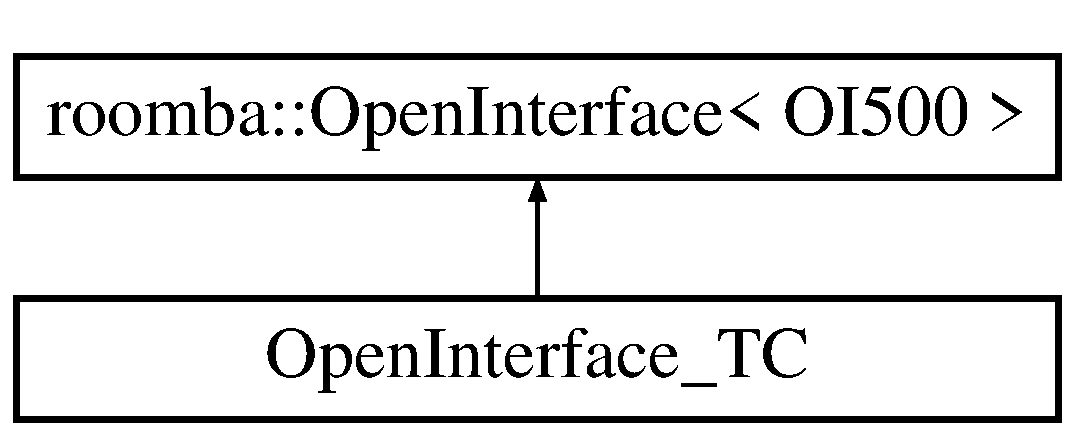
\includegraphics[height=2.000000cm]{class_open_interface___t_c}
\end{center}
\end{figure}
\subsection*{Additional Inherited Members}


The documentation for this class was generated from the following file\+:\begin{DoxyCompactItemize}
\item 
/\+Users/zachary\+\_\+fields/\+Development/bitbucket/irobot-\/roomba-\/500-\/series-\/sdk/gtest/gtest\+\_\+\+O\+I.\+cpp\end{DoxyCompactItemize}

\hypertarget{structroomba_1_1state_1_1sensor__data__t}{\section{roomba\+:\+:state\+:\+:sensor\+\_\+data\+\_\+t Struct Reference}
\label{structroomba_1_1state_1_1sensor__data__t}\index{roomba\+::state\+::sensor\+\_\+data\+\_\+t@{roomba\+::state\+::sensor\+\_\+data\+\_\+t}}
}


Data structure to overlay sensor blob.  




{\ttfamily \#include $<$state.\+h$>$}

\subsection*{Public Attributes}
\begin{DoxyCompactItemize}
\item 
\hypertarget{structroomba_1_1state_1_1sensor__data__t_affcf5db7ad47768ec74b821574e0a04a}{uint8\+\_\+t {\bfseries bumps\+\_\+and\+\_\+wheel\+\_\+drops}}\label{structroomba_1_1state_1_1sensor__data__t_affcf5db7ad47768ec74b821574e0a04a}

\item 
\hypertarget{structroomba_1_1state_1_1sensor__data__t_a42c2a710f160135bb2e80fdf74e7af96}{uint8\+\_\+t {\bfseries wall}}\label{structroomba_1_1state_1_1sensor__data__t_a42c2a710f160135bb2e80fdf74e7af96}

\item 
\hypertarget{structroomba_1_1state_1_1sensor__data__t_afa5ec5b7bb9c149bd3c526cf6626a402}{uint8\+\_\+t {\bfseries cliff\+\_\+left}}\label{structroomba_1_1state_1_1sensor__data__t_afa5ec5b7bb9c149bd3c526cf6626a402}

\item 
\hypertarget{structroomba_1_1state_1_1sensor__data__t_a60420d52300448bbd0f1a743ef0b4b6d}{uint8\+\_\+t {\bfseries cliff\+\_\+front\+\_\+left}}\label{structroomba_1_1state_1_1sensor__data__t_a60420d52300448bbd0f1a743ef0b4b6d}

\item 
\hypertarget{structroomba_1_1state_1_1sensor__data__t_aa4603df2ce86b3b46f663b51d78b96aa}{uint8\+\_\+t {\bfseries cliff\+\_\+front\+\_\+right}}\label{structroomba_1_1state_1_1sensor__data__t_aa4603df2ce86b3b46f663b51d78b96aa}

\item 
\hypertarget{structroomba_1_1state_1_1sensor__data__t_a3fe1e6b6b8da2e5c29ccfa141e2d5b97}{uint8\+\_\+t {\bfseries cliff\+\_\+right}}\label{structroomba_1_1state_1_1sensor__data__t_a3fe1e6b6b8da2e5c29ccfa141e2d5b97}

\item 
\hypertarget{structroomba_1_1state_1_1sensor__data__t_a19de507bd6844a9cd8e57a2948235ee2}{uint8\+\_\+t {\bfseries virtual\+\_\+wall}}\label{structroomba_1_1state_1_1sensor__data__t_a19de507bd6844a9cd8e57a2948235ee2}

\item 
\hypertarget{structroomba_1_1state_1_1sensor__data__t_aa639f842f6a7af27e19e747af18a5497}{uint8\+\_\+t {\bfseries motor\+\_\+overcurrents}}\label{structroomba_1_1state_1_1sensor__data__t_aa639f842f6a7af27e19e747af18a5497}

\item 
\hypertarget{structroomba_1_1state_1_1sensor__data__t_ab0e41664bc347371ca9acc99f7a92945}{uint8\+\_\+t {\bfseries dirt\+\_\+detect}}\label{structroomba_1_1state_1_1sensor__data__t_ab0e41664bc347371ca9acc99f7a92945}

\item 
\hypertarget{structroomba_1_1state_1_1sensor__data__t_ab7ab6ec7eefc8056ff0f93667882f8c2}{uint8\+\_\+t {\bfseries reserved\+\_\+1}}\label{structroomba_1_1state_1_1sensor__data__t_ab7ab6ec7eefc8056ff0f93667882f8c2}

\item 
\hypertarget{structroomba_1_1state_1_1sensor__data__t_a67ba8895c9f340f6132b79661eedb87e}{uint8\+\_\+t {\bfseries infrared\+\_\+character\+\_\+omni}}\label{structroomba_1_1state_1_1sensor__data__t_a67ba8895c9f340f6132b79661eedb87e}

\item 
\hypertarget{structroomba_1_1state_1_1sensor__data__t_aa0fcb04b4a3d014f9a7c4efa3e77e630}{uint8\+\_\+t {\bfseries buttons}}\label{structroomba_1_1state_1_1sensor__data__t_aa0fcb04b4a3d014f9a7c4efa3e77e630}

\item 
\hypertarget{structroomba_1_1state_1_1sensor__data__t_ab544411ae16f10d5e8b83acb17b10037}{uint16\+\_\+t {\bfseries distance}}\label{structroomba_1_1state_1_1sensor__data__t_ab544411ae16f10d5e8b83acb17b10037}

\item 
\hypertarget{structroomba_1_1state_1_1sensor__data__t_adf1e30f57406b9c4c87e916110652d4d}{uint16\+\_\+t {\bfseries angle}}\label{structroomba_1_1state_1_1sensor__data__t_adf1e30f57406b9c4c87e916110652d4d}

\item 
\hypertarget{structroomba_1_1state_1_1sensor__data__t_a44ab2d7044039c6ecdb9357adb971f2d}{uint8\+\_\+t {\bfseries charging\+\_\+state}}\label{structroomba_1_1state_1_1sensor__data__t_a44ab2d7044039c6ecdb9357adb971f2d}

\item 
\hypertarget{structroomba_1_1state_1_1sensor__data__t_a017b7952107891423f80adacc9813381}{uint16\+\_\+t {\bfseries voltage}}\label{structroomba_1_1state_1_1sensor__data__t_a017b7952107891423f80adacc9813381}

\item 
\hypertarget{structroomba_1_1state_1_1sensor__data__t_a98eea7421e0ebe4c1906410265255e31}{uint16\+\_\+t {\bfseries current}}\label{structroomba_1_1state_1_1sensor__data__t_a98eea7421e0ebe4c1906410265255e31}

\item 
\hypertarget{structroomba_1_1state_1_1sensor__data__t_ac9686789c24394b0315e56c745a11a96}{uint8\+\_\+t {\bfseries temperature}}\label{structroomba_1_1state_1_1sensor__data__t_ac9686789c24394b0315e56c745a11a96}

\item 
\hypertarget{structroomba_1_1state_1_1sensor__data__t_ac4858e88a2550903f75ca8ab21f12ba2}{uint16\+\_\+t {\bfseries battery\+\_\+charge}}\label{structroomba_1_1state_1_1sensor__data__t_ac4858e88a2550903f75ca8ab21f12ba2}

\item 
\hypertarget{structroomba_1_1state_1_1sensor__data__t_af6ab62e4408020c91f8cce7695f935ad}{uint16\+\_\+t {\bfseries battery\+\_\+capacity}}\label{structroomba_1_1state_1_1sensor__data__t_af6ab62e4408020c91f8cce7695f935ad}

\item 
\hypertarget{structroomba_1_1state_1_1sensor__data__t_a02a2ba5c6785eb6d664240c015248309}{uint16\+\_\+t {\bfseries wall\+\_\+signal}}\label{structroomba_1_1state_1_1sensor__data__t_a02a2ba5c6785eb6d664240c015248309}

\item 
\hypertarget{structroomba_1_1state_1_1sensor__data__t_a8a6545f242e48729917bdd7401e420f6}{uint16\+\_\+t {\bfseries cliff\+\_\+left\+\_\+signal}}\label{structroomba_1_1state_1_1sensor__data__t_a8a6545f242e48729917bdd7401e420f6}

\item 
\hypertarget{structroomba_1_1state_1_1sensor__data__t_a9b5842f91956ceb120aecb447d77a217}{uint16\+\_\+t {\bfseries cliff\+\_\+front\+\_\+left\+\_\+signal}}\label{structroomba_1_1state_1_1sensor__data__t_a9b5842f91956ceb120aecb447d77a217}

\item 
\hypertarget{structroomba_1_1state_1_1sensor__data__t_ae494bbdf511947e90ca507169e301d80}{uint16\+\_\+t {\bfseries cliff\+\_\+front\+\_\+right\+\_\+signal}}\label{structroomba_1_1state_1_1sensor__data__t_ae494bbdf511947e90ca507169e301d80}

\item 
\hypertarget{structroomba_1_1state_1_1sensor__data__t_ab13bfedf43028cdafa82b92d1c4fba34}{uint16\+\_\+t {\bfseries cliff\+\_\+right\+\_\+signal}}\label{structroomba_1_1state_1_1sensor__data__t_ab13bfedf43028cdafa82b92d1c4fba34}

\item 
\hypertarget{structroomba_1_1state_1_1sensor__data__t_a99c228bd5e6a96a5ede4691ddf6b24d8}{uint8\+\_\+t {\bfseries reserved\+\_\+2}}\label{structroomba_1_1state_1_1sensor__data__t_a99c228bd5e6a96a5ede4691ddf6b24d8}

\item 
\hypertarget{structroomba_1_1state_1_1sensor__data__t_a8da77343aa05916214edb577be4116d9}{uint16\+\_\+t {\bfseries reserved\+\_\+3}}\label{structroomba_1_1state_1_1sensor__data__t_a8da77343aa05916214edb577be4116d9}

\item 
\hypertarget{structroomba_1_1state_1_1sensor__data__t_a10fa8ec7b406eb4e2c163dbfaea01d55}{uint8\+\_\+t {\bfseries charging\+\_\+sources\+\_\+available}}\label{structroomba_1_1state_1_1sensor__data__t_a10fa8ec7b406eb4e2c163dbfaea01d55}

\item 
\hypertarget{structroomba_1_1state_1_1sensor__data__t_a878004b9b3ff1f7ae7d324d7a0132214}{uint8\+\_\+t {\bfseries oi\+\_\+mode}}\label{structroomba_1_1state_1_1sensor__data__t_a878004b9b3ff1f7ae7d324d7a0132214}

\item 
\hypertarget{structroomba_1_1state_1_1sensor__data__t_a0047e6201366b8fe897890d0e57591c7}{uint8\+\_\+t {\bfseries song\+\_\+number}}\label{structroomba_1_1state_1_1sensor__data__t_a0047e6201366b8fe897890d0e57591c7}

\item 
\hypertarget{structroomba_1_1state_1_1sensor__data__t_aae42b69a5a11cb7b5efd05f0cb5fbd4f}{uint8\+\_\+t {\bfseries song\+\_\+playing}}\label{structroomba_1_1state_1_1sensor__data__t_aae42b69a5a11cb7b5efd05f0cb5fbd4f}

\item 
\hypertarget{structroomba_1_1state_1_1sensor__data__t_af9fdeec636094cbd6f397c52534c2e66}{uint8\+\_\+t {\bfseries number\+\_\+of\+\_\+stream\+\_\+packets}}\label{structroomba_1_1state_1_1sensor__data__t_af9fdeec636094cbd6f397c52534c2e66}

\item 
\hypertarget{structroomba_1_1state_1_1sensor__data__t_ad2798fbc0b44c4551d45d8e82c07de6f}{uint16\+\_\+t {\bfseries requested\+\_\+velocity}}\label{structroomba_1_1state_1_1sensor__data__t_ad2798fbc0b44c4551d45d8e82c07de6f}

\item 
\hypertarget{structroomba_1_1state_1_1sensor__data__t_a30c5d4af100001365a1e913694e70974}{uint16\+\_\+t {\bfseries requested\+\_\+radius}}\label{structroomba_1_1state_1_1sensor__data__t_a30c5d4af100001365a1e913694e70974}

\item 
\hypertarget{structroomba_1_1state_1_1sensor__data__t_afc799bfff2d3fbc99d48046ebce3c54c}{uint16\+\_\+t {\bfseries requested\+\_\+right\+\_\+velocity}}\label{structroomba_1_1state_1_1sensor__data__t_afc799bfff2d3fbc99d48046ebce3c54c}

\item 
\hypertarget{structroomba_1_1state_1_1sensor__data__t_a6c1a2fe57a6e470c5712cea20577516e}{uint16\+\_\+t {\bfseries requested\+\_\+left\+\_\+velocity}}\label{structroomba_1_1state_1_1sensor__data__t_a6c1a2fe57a6e470c5712cea20577516e}

\item 
\hypertarget{structroomba_1_1state_1_1sensor__data__t_a2a733a51ed71bc46862371ff8f14a608}{uint16\+\_\+t {\bfseries right\+\_\+encoder\+\_\+counts}}\label{structroomba_1_1state_1_1sensor__data__t_a2a733a51ed71bc46862371ff8f14a608}

\item 
\hypertarget{structroomba_1_1state_1_1sensor__data__t_a6035187d56dac6c87412a4c046d15f68}{uint16\+\_\+t {\bfseries left\+\_\+encoder\+\_\+counts}}\label{structroomba_1_1state_1_1sensor__data__t_a6035187d56dac6c87412a4c046d15f68}

\item 
\hypertarget{structroomba_1_1state_1_1sensor__data__t_abadede4ec67fcf516d8a7cea886511c4}{uint8\+\_\+t {\bfseries light\+\_\+bumper}}\label{structroomba_1_1state_1_1sensor__data__t_abadede4ec67fcf516d8a7cea886511c4}

\item 
\hypertarget{structroomba_1_1state_1_1sensor__data__t_ab823b00555186b149292037066709f38}{uint16\+\_\+t {\bfseries light\+\_\+bump\+\_\+left\+\_\+signal}}\label{structroomba_1_1state_1_1sensor__data__t_ab823b00555186b149292037066709f38}

\item 
\hypertarget{structroomba_1_1state_1_1sensor__data__t_a0cafaa751c44698b6baab0beb8dae76a}{uint16\+\_\+t {\bfseries light\+\_\+bump\+\_\+front\+\_\+left\+\_\+signal}}\label{structroomba_1_1state_1_1sensor__data__t_a0cafaa751c44698b6baab0beb8dae76a}

\item 
\hypertarget{structroomba_1_1state_1_1sensor__data__t_ad67229cd78f37ef4beb61159c1b8ca23}{uint16\+\_\+t {\bfseries light\+\_\+bump\+\_\+center\+\_\+left\+\_\+signal}}\label{structroomba_1_1state_1_1sensor__data__t_ad67229cd78f37ef4beb61159c1b8ca23}

\item 
\hypertarget{structroomba_1_1state_1_1sensor__data__t_a24abc6e870b0853fc41113b138989da4}{uint16\+\_\+t {\bfseries light\+\_\+bump\+\_\+center\+\_\+right\+\_\+signal}}\label{structroomba_1_1state_1_1sensor__data__t_a24abc6e870b0853fc41113b138989da4}

\item 
\hypertarget{structroomba_1_1state_1_1sensor__data__t_accb10bcc1ff53745ef887d32375b7b74}{uint16\+\_\+t {\bfseries light\+\_\+bump\+\_\+front\+\_\+right\+\_\+signal}}\label{structroomba_1_1state_1_1sensor__data__t_accb10bcc1ff53745ef887d32375b7b74}

\item 
\hypertarget{structroomba_1_1state_1_1sensor__data__t_afee4bff605d289941ee87c71283ad7d2}{uint16\+\_\+t {\bfseries light\+\_\+bump\+\_\+right\+\_\+signal}}\label{structroomba_1_1state_1_1sensor__data__t_afee4bff605d289941ee87c71283ad7d2}

\item 
\hypertarget{structroomba_1_1state_1_1sensor__data__t_a3c84f3e8b2a8fdc8ec8722639e7b0ee1}{uint8\+\_\+t {\bfseries infrared\+\_\+character\+\_\+left}}\label{structroomba_1_1state_1_1sensor__data__t_a3c84f3e8b2a8fdc8ec8722639e7b0ee1}

\item 
\hypertarget{structroomba_1_1state_1_1sensor__data__t_a8093e19808bf33e5b628effa00d1eded}{uint8\+\_\+t {\bfseries infrared\+\_\+character\+\_\+right}}\label{structroomba_1_1state_1_1sensor__data__t_a8093e19808bf33e5b628effa00d1eded}

\item 
\hypertarget{structroomba_1_1state_1_1sensor__data__t_a29d4a11a443945d84cc1e49a83b74c4d}{uint16\+\_\+t {\bfseries left\+\_\+motor\+\_\+current}}\label{structroomba_1_1state_1_1sensor__data__t_a29d4a11a443945d84cc1e49a83b74c4d}

\item 
\hypertarget{structroomba_1_1state_1_1sensor__data__t_a58c16c028125e0ab9eede4f57ac3b4e8}{uint16\+\_\+t {\bfseries right\+\_\+motor\+\_\+current}}\label{structroomba_1_1state_1_1sensor__data__t_a58c16c028125e0ab9eede4f57ac3b4e8}

\item 
\hypertarget{structroomba_1_1state_1_1sensor__data__t_a5113576c63aeb578ee03701df5c53ed1}{uint16\+\_\+t {\bfseries main\+\_\+brush\+\_\+motor\+\_\+current}}\label{structroomba_1_1state_1_1sensor__data__t_a5113576c63aeb578ee03701df5c53ed1}

\item 
\hypertarget{structroomba_1_1state_1_1sensor__data__t_a42ec2f526cc3bc01ec9c1eba7c0ab7c1}{uint16\+\_\+t {\bfseries side\+\_\+brush\+\_\+motor\+\_\+current}}\label{structroomba_1_1state_1_1sensor__data__t_a42ec2f526cc3bc01ec9c1eba7c0ab7c1}

\item 
\hypertarget{structroomba_1_1state_1_1sensor__data__t_a427c36b559be00c0afcd6bfa98c0c62e}{uint8\+\_\+t {\bfseries stasis}}\label{structroomba_1_1state_1_1sensor__data__t_a427c36b559be00c0afcd6bfa98c0c62e}

\end{DoxyCompactItemize}


\subsection{Detailed Description}
Data structure to overlay sensor blob. 

The data structure provides field name access to the sensor data returned by the Roomba. \begin{DoxyNote}{Note}
This data structure must be given the packed attribute, due the fact the data is not divisible into even blocks of 8, 16, 32 or 64. 
\end{DoxyNote}
\begin{DoxySeeAlso}{See also}
\hyperlink{classroomba_1_1_open_interface_aa676703a4c79547397eaa89ddb9e207c}{Open\+Interface\+::sensors} 

\hyperlink{classroomba_1_1_open_interface_a4a7308a7119c6a462389d9ffa3785f87}{Open\+Interface\+::query\+List} 

\hyperlink{classroomba_1_1_open_interface_af7a1adea482ac71fa9057842a955af6e}{Open\+Interface\+::stream} 
\end{DoxySeeAlso}


The documentation for this struct was generated from the following file\+:\begin{DoxyCompactItemize}
\item 
/\+Users/zachary\+\_\+fields/\+Development/bitbucket/irobot-\/roomba-\/sdk/hardware/state.\+h\end{DoxyCompactItemize}

%--- End generated contents ---

% Index
\newpage
\phantomsection
\addcontentsline{toc}{chapter}{Index}
\printindex

\end{document}
